
\chapter{光的反射和折射}

光学是物理学中发展得最早的分支之一,远在二千四百
多年前我国的墨翟(公元前468—376)及其弟子们所著的《墨
经》一书,就记载了光的直线传播、光的反射等现象,称得上是
世界上最早的光学著作。宋代沈括(1031—1095)在《梦溪笔
谈》中记载了极为丰富的光学知识。后来,各国科学家们发明
了眼镜、望远镜、显微镜、照相机等光学仪器,并对光的本性进
行了研究,把光学应用于生产技术和生活中。本世纪六十年代
激光出现以后,光学的研究和应用有了新的发展,光学与其他
科学技术紧密结合,在各个领域中得到了广泛的应用,成为现
代物理学和现代科学技术的重要前沿之一。

在中学我们主要学习光的传播和光的本性的知识。

\section{光的直线传播}
\subsection{光源}

在漆黑的屋子里,我们什么也看不见。如果点上
一盏灯,就可以看见灯,也可以看见屋子里的桌、椅、墙壁等。
我们能够看见灯的发光部分,是因为它发出的光进入了我们
的眼睛,引起了视觉,我们能够看见桌、椅、墙壁等,是因为它
们反射光。

电灯、蜡烛、太阳、萤火虫等,能够自行发光,我们把这样
的物体叫做\textbf{光源}。

光具有能量,它可以使物体变热,使照相底片感光,使光
电池供电,光源发光要消耗其他形式的能,由其他形式的能
转化成光能。电灯发光消耗了电能,蜡烛发光消耗了化学能,
太阳发光消耗了太阳内部的原子能。

\subsection{光的直线传播}

我们知道,光是沿直线传播的。把一块
有窄缝的硬纸板挡在光源前面,可以看到,从窄缝射出的光束
沿直线前进(图5.1)。
\begin{figure}[htp]\centering
    \includegraphics[scale=.6]{fig/5-1.png}
    \caption{光沿直线传播}
    \end{figure}

在研究光的传播规律时,为了方便,常用一条直线来表示
光的传播方向,这样的直线,叫做\textbf{光线}。光线是个很有用的概
念,利用光线我们就可以用几何学的方法来研究光的传播问
题,应该注意的是,光线并不是实际存在的东西,实际中只
能得到很窄的光束,不能得到象几何线那样的光线,正如质
点是物体的抽象一样,光线是光束的抽象。

自然界中的许多光现象,例如影、日食、月食等,都是光沿
直线传播而产生的。日常生活中,我们也经常运用光沿直线
传播的性质,例如,知道了一个发光点发出的两条光线的方
向,根据光沿直线传播的性质,就可以确定这个发光点的位
置;照图5.2那样,把两条光线向反方向延长,它们的交点的
位置就是发光点的位置。人的眼睛在观察物体时,就是利用
这种方法来确定物体的位置的。根据从铅笔尖射到眼睛的两
条光线,人们判断铅笔尖的位置在这两条光线反方向延长线
的交点(图5.3)。
\begin{figure}[htp]
    \centering
    \begin{minipage}[t]{0.48\textwidth}
    \centering
\begin{tikzpicture}[>=latex]
\node at (0,0){\Sun};
\node at (-.5,0){$S$};
\draw[dashed] (0,0)--(15:2)node[above]{$A$};
\draw[dashed] (0,0)--(-15:2)node[below]{$C$};
\draw[->](15:2)--(15:3.5)node[above]{$B$};
\draw[->](-15:2)--(-15:3.5)node[below]{$D$};


\end{tikzpicture}
    \caption{利用光线
    确定物体的位置}
    \end{minipage}
    \begin{minipage}[t]{0.48\textwidth}
    \centering
    \includegraphics[scale=.6]{fig/5-3.png}
    \caption{眼睛根据光的直线传播确定物体的位置}
    \end{minipage}
    \end{figure}

\section{光的速度}
光从光源发出,以有限的速度向外传播。光传播得很快,
在日常接触到的距离内,光从光源到达我们的眼睛所用的时
间很短,凭感觉根本无法察觉出来,所以在历史上很长一段时
间里,人们一直认为光的传播是不需要时间的,直到十七世
纪才发现光是以有限的速度传播的。

1607年伽利略最早做了测定光速的尝试.让两个实验
者在夜间每人各带一盏遮蔽着的灯,站在相距约1.6千米的
两个山顶上。第一个实验者先打开灯,同时记下开灯的时间。
第二个实验者看到传来的灯光后,立刻打开自己的灯。第一
个实验者看到第二个实验者的灯光后,再立刻记下时间,然
后根据记下的时间间隔和两山顶间的距离计算光的传播速
度。这种测量光速的方法原理虽然正确,却没有得出什么实
验结果。这是因为光的速度很大,在相距约1.6千米的两山
顶间来回一次,所用的时间大约只有十万分之一秒,用这种简
单粗糙的方法根本不能测出这样短的时间来。伽利略测定光
速的实验虽然失败了,但是它表明了光的速度是很大的,在不
太长的距离上不能用粗糙的计时方法测量出来。
要测定光速,必须利用很大的距离,或者用精巧的办法准
确地测量出很短的时间间隔。伽利略以后的学者们正是沿着
这两个方向探求测定光速的方法的。

\begin{figure}[htp]\centering
    \includegraphics[scale=.6]{fig/5-4.png}
    \caption{罗默用天文观测的方法测定光速的示意图。
    设卫星第一次食毕,地球在$C$点,卫星绕木
    星公转一周,第二次食毕,地球在$D$点,因此
    光要多传播一段距离$\ell$才能到达地球。}
    \end{figure}

1676年丹麦天文学家罗默(1644—1710)用天文观测的
方法,发现了光是以有限的速度传播的。罗默是在观测木星
的卫星食的过程中得到这一发现的。如图5.4所示,木星的
卫星绕木星每转一周都要消失在木星的影内一次,即发生一
次卫星食,相继的两次卫星食间隔的时间,就是这个卫星绕
木星公转一周的周期,这个周期不大,约为1.75天。罗默在
整年中连续观测了卫星的公转周期,发现这个周期不是恒定
的。当地球在绕日运行的轨道上远离木星而去时,即地球在
图中所示由$A$运行到$B$的半年里,卫星的周期长;当地球在轨
道上向着木星运行时,即地球在由$B$运行到$A$的半年里,周
期短。罗默认为,这是由于光以有限的速度传播而造成的。
当地球远离木屋运动时,卫星第二次食毕,从木星的影中出
来,卫星发出的光到达地球要多传播一段距离,所以观测到的
周期长;当地球向着木星运动时,光到达地球要少传播一段距
离,所以观测到的周期短。周期长或短的数值跟光速的大小
有关系。利用罗默观测到的数据和地球绕日运行的轨道直径,
可以计算出光速的大小。

为了在地面上不太长的距离内测定光速,科学家们设计
了各种巧妙的实验方法,以便准确地测出很短的时间间隔,下
面我们简略地介绍一下美国物理学家迈克耳孙(1852—1931)
的旋转棱镜法。
\begin{figure}[htp]\centering
    \includegraphics[scale=.6]{fig/5-5.png}
    \caption{迈克耳孙测定光速实验的示意图}
    \end{figure}

迈克耳孙选择了两个山峰,测出两山峰间的距离,在第一
个山峰上安装一个强光源$S$和一个正八面棱镜$A$(图5.5),光
源$S$发出的光,经过狭缝射到八面镜$A$的面1上,反射后射到
放置在另一个山峰上的凹镜$B$上,经平面镜$M$反射后,再由凹
镜$B$反射回第一个山峰。如果八面镜静止不动,反射回来的
光就射到八面镜的另一个面3上,经面3反射后,通过望远镜
$C$进入观察者的眼中,看到光源$S$的像。

如果使八面镜转动,那么光经凹镜$B$反射回来时,八面镜
的面3已经偏离了原来的方向,经面3反射后的光将不再进
入望远镜中,观察者就观察不到光源$S$的像了。适当调节八
面镜的转速,使反射回来的光到达八面镜时,八面镜恰好转过
$1/8$转,这时面2正好转到原来面3所在的位置,经面2反射后
的光就可以进入望远镜中,观察者就可以重新看到S的像。根
据八面镜转过$1/8$
转所用的时间和两山峰间的距离,就可以算
出光在空气里的速度。迈克耳孙经过校正,得出光在真空中
的速度$c=299796{\rm km}/{\rm s}$。

1970年以后,开始利用激光测量光速,这种测量方法的
原理是测出激光的波长$\lambda$和频率$\nu$,利用$c=\lambda\nu$ 计算得出光
速$c$来(关于光是一种波动的知识将在下一章中学习),激光
测速法大大提高了测量的精确度,根据1975年第15届国际
计量大会决议,真空中的光速值定为
$$c=299792458\ms$$
在通常的计算中,可取$c=3.00\x10^8\ms$。

\subsection*{练习一}
\begin{enumerate}
    \item 在图5.6中,$S$是一个点光源,$AB$是物体,$E$是屏
幕,试画出$AB$在屏幕上所成
的影的范围。
\begin{figure}[htp]
	\centering
\begin{tikzpicture}
\node at (-1.1,0) {$S$};
\node at (-.7,0){\Sun};
\draw (1, -.5)node[below]{$B$}--(1,.5)node [above]{$A$};
\draw (3, -2)--(3,2)node [above]{$E$};
\end{tikzpicture}
	\caption{}
\end{figure}


\item 为什么在发生日食的
时候,有的地方能看到日全食,
有的地方只能看到日偏食?在
什么情况下能看到日环食?画
出地球、月球和太阳位置的简图来解释发生这几种日食的原
因。
\item 现在需要知道学校里升国旗的旗杆的高度,你能否
利用光的直线传播知识想出一种测量的办法来?
\item 边长5厘米的正方形卡片,放在小灯泡正前方15厘
米的地方,在卡片后方放一个跟卡片平行的纸屏,纸屏距卡片
15厘米,卡片在屏上的影是什么形状?面积多大?
\item 在迈克耳孙测定光速的一次实验中,测得两山峰间
的距离为35373.21米,八面镜的旋转速度为528转/秒,试利
用这些数据算出光在空气中的速度。
\end{enumerate}

\section{光的反射~~平面镜}
\subsection{光的反射}
前面讲的光沿直线传播,是就光在同一种媒
质里的传播而言的,当光从一种媒质射入另一种媒质,例如
从空气射入玻璃或水里时,在两种媒质的分界面上,光将改变
传播方向,一部分光被反射回原来的媒质中,这种现象叫做
\textbf{光的反射}。

我们在初中学过,光的反射遵守下面的\textbf{反射定律}:

\begin{enumerate}
    \item 反射光线跟入射光线和法线在同一平面上,反射光
线和入射光线分居在法线的两侧;
\item 反射角等于入射角。
\end{enumerate}

根据光的反射定律,如果使光线沿着反射光线的路径射
到界面上,这时的反射光线一定会沿着原来入射光线的路径
射出,就是说,反射时光路是可逆的。

平滑的表面,例如镜面、平静的水面等,能使平行的入射
光线沿同一方向平行地反射出去(图5.8),这时只在这个方
向有反射光线,其他方向没有反射光线,这样的反射叫做镜面
反射。
\begin{figure}[htp]
    \centering
    \begin{minipage}[t]{0.48\textwidth}
    \centering
    \begin{tikzpicture}[>=Stealth, scale=1]
        \draw (-2,0)--(2,0);
    \draw(0,0)--(0,3)node [above]{法线};
    \draw[very thick] (135:3)node [above]{入射光线}--(0,0);  \draw[very thick] (45:3)node [above]{反射光线}--(0,0);	
    \draw[->] (135:3)--(135:1.5);  \draw[->] (0,0)--(45:1.5);
    \draw (0,.65) arc (90:45:.65) node [above]{$r$};	
    \draw (0,.5) arc (90:135:.5)node [above]{$i$};	
        \end{tikzpicture}
    \caption{光的反射}
    \end{minipage}
    \begin{minipage}[t]{0.48\textwidth}
    \centering
        \begin{tikzpicture}[>=stealth, xscale=.6]
    
    \foreach \x in {1,2,3,4,5}
    {
        \draw[->, very thick] (\x,0)--(\x+3,3);
        \draw[very thick] (\x,0)--(\x-3,3);
        \draw[<-, very thick] (\x-2,2)--(\x-3,3);
    }
    
    \fill [pattern=north east lines] (-1,-.25) rectangle (7,0);
        \draw (-1,0)--(7,0);
        \end{tikzpicture}
    \caption{镜面反射}
    \end{minipage}
    \end{figure}

如果表面是粗糙不平的,那么沿同一方向射到面上的光
线将向不同的方向反射(图5.9),这样的反射叫做漫反射。我
们能从不同方向看见本身不发光的物体,比如看见书上的字,
就是因为光在纸面上发生漫反射的缘故。
\begin{figure}[htp]
    \centering
    \begin{minipage}[t]{0.48\textwidth}
    \centering
    \includegraphics[scale=1.4]{fig/5-9.pdf}
    \caption{漫反射}
    \end{minipage}
    \begin{minipage}[t]{0.48\textwidth}
    \centering
    \includegraphics[scale=.6]{fig/5-10.png}
    \caption{平面镜成虚像}
    \end{minipage}
    \end{figure}

    \subsection{平面镜}

    日常生活中用的镜子都是平面镜,从镜子里可
    以看到镜前物体的像。平面镜里的像是怎样产生的呢?

    在图5.10中,$M$是平面镜,一支蜡烛位于镜前。为了研
    究蜡烛所成的像,我们先来研究烛焰上的一点$S$在镜中的像。
    从$S$射向镜面的光线中,任取两条光线$SA$和$SB$,这两条光
    线被镜面反射后,分别沿着$AC$和$BE$的方向进入眼睛。发
    光点虽然在$S$,但是我们根据光沿直线传播的经验,认为光线
    $AC$和$BE$是从它们的反向延长线的交点$S'$射来的,从$S$点
    发出的其他光线经镜面反射后,反向延长线也通过$S'$点(请
    同学们自己证明一下),$S'$就是$S$在平面镜中的像,因为光
    线实际上不是从$S'$发出的,$S'$并不是光线的实际交点,而是
    光线的反向延长线的交点,所以光学中把这样的像叫做\textbf{虚像}。

    从$S$点发出的垂直于镜面的光线$SO$,经镜面反射后,沿
    原路返回。这条反射光线的反向延长线也通过$S'$点。根据
    反射定律,可以证明直角三角形$SAO$和$S'AO$全等,所以$S'O=SO$。
    就是说,像到镜面的距离等于物到镜面的距离。像和
    物对镜面是对称的。

    整个蜡烛可以看成是由许多点组成的,每个点都在镜子
    里产生一个虚像,这许多点的像就组成了蜡烛的虚像。

    平面镜除了在生活中作镜
    子用,还广泛应用在各种仪器
    中。例如,在高一讲过的显示微
    小形变的装置中,在库仑扭秤
    装置中,都装有平面镜,用反射
    光线把微小效应放大。潜望镜
    中用平面镜来改变光线的行进
    方向(图5.11)。
    \begin{figure}[htp]\centering
        \includegraphics[scale=.6]{fig/5-11.png}
        \caption{潜望镜示意图}
    \end{figure}

\subsection*{练习二}
\begin{enumerate}
    \item 甲乙二人面对着镜子,甲能从镜中看到乙的眼睛,乙
    是否也能看到甲的眼睛?说明理由。
    \item 在图5.11的潜望镜中,两平面镜倾斜的角度是多大?
    \item 晚上在灯下看书,如果书的纸面很光滑,有时会看到
    纸面上发出刺眼的光泽,为什么会出现这种现象?怎样消除
    它?
    \item 如图5.12所示,两个平面镜互相垂直,在跟这两个
    镜面垂直的平面内,有一条入射光线$AB$,经两个镜面反射后,
    沿$CD$方向射出,试证明不论光线$AB$以多大的入射角射入,反射光线$CD$都平行于$AB$射出。
    
    根据上面的现象,在六十年代,曾制作了由三块平面镜组
    成的反射器,由登月宇航员带到了月球上。这三块平面镜象
    房子里的墙角那样,彼此相交成直角,能把任何方向射到镜面
    上的光线逆着原方向反射回去。精确测出激光从地球射到这
    个反射器再返回地球的时间,再利用光速值就可以算出月球
    到地球的距离,
    \item 图5.13中,$M$是一个平面镜,$S$是光源,通过狭缝使
    光线射到镜面上,$M$的位置,最初是与$S$射来的光线垂直,这
    时反射光线射在标尺的零刻度上;当$M$转动一角度后,反射光
    线射到标尺的$n$刻度上。如果标尺到镜$M$的距离为$\ell$,且$\ell\gg on$,
    求$M$转动的角度是多大。
    \item 有的镜子照出的像会变形,这是什么原因?
    \begin{figure}[htp]
        \centering
        \begin{minipage}[t]{0.48\textwidth}
        \centering
        \includegraphics[scale=.6]{fig/5-12.png}
        \caption{}
        \end{minipage}
        \begin{minipage}[t]{0.48\textwidth}
        \centering
        \includegraphics[scale=.6]{fig/5-13.png}
        \caption{}
        \end{minipage}
        \end{figure}
\end{enumerate}
    
\section{球面镜}
反射面是球面一部分的镜叫做\textbf{球面镜}。用球面的内表面
作反射面的叫做\textbf{凹镜},用球面的外表面作反射面的叫做\textbf{凸镜}。

\subsection{球面镜的焦点和焦距}

凹镜对光线起会聚作用。射到凹
镜上的平行光线,被反射后会聚于一点(图5.14甲),这一点叫
做凹镜的焦点,通常用$F$表示。如果把一张纸放在焦点,纸上
会出现一个很亮的光点。凹镜的焦点是反射光线的实际会聚
点,是实焦点。
\begin{figure}[htp]\centering
\begin{minipage}[t]{0.48\textwidth}
\centering
\begin{tikzpicture}[>=latex, scale=1.5]
            \fill [pattern=north east lines] (2,-1)--(2.2,-1) to [bend left=-30] (2.2,1) --(2,1) to [bend left=30](2,-1);
            \draw [thick](2,1) to [bend left=30] (2,-1);
        \foreach \x in {-.8,-.4,0,...,.8}
        {
            \draw[->] (0,\x)--(0.5,\x);
        }    
        \draw  (0,-.8)--(2.1,-.8)--(1,0)--(.95/2,.4);\draw  (0,.8)--(2.1,.8)--(1,0)--(.95/2,-.4);
        \draw  (0,-.4)--(2.2,-.4)--(1,0)--(.9/2,.2);\draw  (0,.4)--(2.2,.4)--(1,0)--(.9/2,-.2);
        \draw  (0,0)--(2.3,0);

        \draw[->](2.1,-.8)--(3.1/2,-.4);  \draw[->](2.1,.8)--(3.1/2,.4);
        \draw[->](2.2,-.4)--(3.2/2,-.2);   \draw[->](2.2,.4)--(3.2/2,.2);
        \draw[->] (2.3,0)--(3.3/2,0);
        \node at (1,0)[above]{$F$};      \node at (2.6,0){$P$};   
        \draw (1,0)[ fill=black] circle (1pt);

        \end{tikzpicture}
\caption*{甲}
\end{minipage}
\begin{minipage}[t]{0.48\textwidth}
\centering
\begin{tikzpicture}[>=latex,scale=1.5]
    \fill [pattern=north east lines] (-2,-1)--(-2.2,-1) to [bend left=30] (-2.2,1) --(-2,1) to [bend left=-30]
    (-2,-1);
\draw [thick](-2.2,1) to [bend left=-30] (-2.2,-1);
\foreach \x in {-.8,-.4,0,...,.8}
        {
            \draw[->] (-4,\x)--(-3.5,\x);
        }    

        \draw(-3.5,-.8)--(-2.3,-.8);\draw(-3.5,-.4)--(-2.45,-.4);
        \draw(-3.5,.4)--(-2.45,.4);\draw(-3.5,.8)--(-2.3,.8);
        \draw(-3.5,0)--(-2.5,0);  \draw[->](-2.5,0)--(-3.2,0);
\draw[dashed] (-2.5,0)--(-1,0)node [below]{$F$}--(0,0)node [right]{$C$};
\draw [dashed](-2.3,-.8)--(-1,0);\draw [dashed](-2.45,-.4)--(-1,0);
\draw [dashed](-2.45,.4)--(-1,0);\draw [dashed](-2.3,.8)--(-1,0);

\draw [->](-2.3,-.8)--(-2.95,-1.2);\draw [->](-2.45,-.4)--(-6.35/2,-.6);
\draw [->](-2.45,.4)--(-6.35/2,.6);\draw [->](-2.3,.8)--(-2.95,1.2);
\node at (-2.7,0)[above]{$P$};
\draw (-1,0)[ fill=black] circle (1pt);

\end{tikzpicture}
\caption*{乙}
\end{minipage}
    \caption{球面镜的焦点和焦距}
    \end{figure}

凸镜对光线起发散作用,射到凸镜上的平行光线,被反
射后变得发散,把反射光线反向延长后,它们将会聚于一点
(图5.14乙),这一点叫做凸镜的焦点,凸镜的焦点不是反射
光线的实际会聚点,是虚焦点。

镜面的中心点$P$叫做球面镜的顶点,连接球心$C$和顶点
$P$的直线叫做主光轴,简称主轴。靠近主轴射向镜面的光线
叫做近轴光线。严格说来,只有平行于主轴的近轴光线经球
面镜反射后,才能会聚于一点,我们这里研究的只限于近轴
光线。

焦点到顶点的距离叫做焦距,通常用$f$表示。对于近轴
光线,球面镜的焦距等于球半径$R$的一半,即$f=R/2$。

利用凹镜对光的会聚作用,人们制造了生活中用的太阳
灶和工业上用的太阳炉,这是利用太阳能的一种重要方法。

反射时光路是可逆的,如果把光源放在凹镜的焦点,那么
从光源射向凹镜的光线,反射后将平行射出。探照灯、汽车头
灯、手电筒等射出的光束比较集中,能够照亮远处的物体,就
是利用了凹镜的这一性质。

凸镜可以用来扩大观察范围.从图5.15可以看出,对于
口径相同的平面镜和凸镜,观察者离镜同样远时,从凸镜观察
到的范围要比平面镜大,用一个口径不太大的凸镜,就能观
察到比较大的范围内的景像,因此,汽车上的观后镜都用
凸镜。

\begin{figure}[htp]\centering
    \includegraphics[scale=.6]{fig/5-15.png}
    \caption{}
    \end{figure}

\subsection{球面镜成像}
球面镜也可以使物体成像,物体离球面镜
的距离不同,所成的像也不同。我们可以用下面的实验来观
察球面镜的成像情况。
\begin{figure}[htp]\centering
    \includegraphics[scale=.6]{fig/5-16.png}
    \caption{凹镜成像\\
    甲:物体位于二倍焦距以外时,成倒立缩小的实像;\\
    乙:物体位于二倍焦距和焦点之间时,成倒立放大的实像;\\
    丙:物体位于焦点以内时,成正立放大的虚像。}
    \end{figure}

如图5.16所示,把一支蜡烛放在凹镜前二倍焦距以外的
地方,用一张透明纸作光屏,在蜡烛和凹镜之间移动光屏,直
到在光屏上出现清晰的蜡烛的像。可以看到,这时的像是倒
立缩小的(图5.16甲)。这个像是由反射光线实际会聚而成
的,能够用光屏接收到,所以光学中把这样的像叫做\textbf{实像}。
把蜡烛向凹镜移近,同时使光屏远离凹镜,当蜡烛位于二
倍焦距以内焦点以外时,从光屏上可以看到倒立放大的实像
(图5.16乙).使蜡灿进一步靠近镜面,当蜡烛位于焦点以内
时,无论怎样移动光屏,都得不到蜡烛的像。这时向镜里看
去,可以看到一个正立放大的像(图5.16丙).这个像不是
由反射光线实际会聚而成的,用光屏接收不到,是虚像。

把蜡烛放在凸镜前的任何位置上,用光屏都接收不到蜡
烛的实像,只能从镜中看到蜡烛的正立缩小的虚像
(图5.17)。
   \begin{figure}[htp]\centering
\begin{tikzpicture}[>=latex, scale=1.5]
    \fill [pattern=north east lines] (2,-1)--(2.2,-1) to [bend left=30] (2.2,1) --(2,1) to [bend left=-30]
    (2,-1);
\draw [thick](2,1) to [bend left=-30] (2,-1);
\draw [dashed] (-3,0)--(4,0);
\node at (3,0) [above]{$F$};
\draw (3,0) [fill=black] circle (1.5pt);

\draw (-2.5,0) rectangle (-2, .5);
\draw (-2.25, .5) to [bend left=30] (-2.25,1) to [bend left=30]  (-2.25, .5);

\draw [dashed](2.5,0) rectangle (2.75, .25);
\draw [dashed](2.625, .25) to [bend left=30] (2.625, .5) to [bend left=30]  (2.625, .25);


\end{tikzpicture}
        \caption{凸镜只能成正立缩小的虚像}
        \end{figure}

\subsection*{练习三}
\begin{enumerate}
    \item 有一个凹镜,要想知道它的焦距,请你想出一个粗略
        测量的方法来。
    \item 比较凹镜和凸镜的成像情况有什么不同。
    \item 有一个凹镜,把它放在你的面前,如果能从镜中看到
        你自己的正立的像,这时凹镜顶点到你的距离是20厘米,那
        么这个凹镜的焦距至少有多大?
    \item 如图5.18所示,$M_1$和$M_2$是两个焦距相等的凹镜,
    其焦距为$f$。要想使平行于主轴的光线$a$能在$M_1$和$M_2$之
    间来回反射,两凹镜的顶点$P_1$
    和$P_2$应相距多远?在图中标出
    两凹镜的焦点$F_1$和$F_2$的位置,
    并画出光线$a$被两凹镜反射的
    光路图。
\end{enumerate}

\begin{figure}[htp]\centering
\begin{tikzpicture}[>=latex]
        \fill [pattern=north east lines] (-2,-1)--(-2.2,-1) to [bend left=30] (-2.2,1) --(-2,1) to [bend left=-30]
        (-2,-1);
\draw [thick](-2,1) to [bend left=-30] (-2,-1);
 
\fill [pattern=north east lines] (2,-1)--(2.2,-1) to [bend left=-30] (2.2,1) --(2,1) to [bend left=30](2,-1);
\draw [thick](2,1) to [bend left=30] (2,-1);
\draw [dashed] (-2.3,0)--(2.3,0);
\node at (-2.1,0)[below]{$P_1$};\node at (2.1,0)[below]{$P_2$};
\node at (-2.2,1)[above]{$M_1$};\node at (2.2,1)[above]{$M_2$};
\draw (-.5,.7)--node[above]{$a$}(2.15,.7);
        \end{tikzpicture}
    \caption{}
    \end{figure}
 
\section{光的折射}
光从空气斜射到玻璃上,在界面上一部分光线发生反射,
回到空气中;另一部分光线射入玻璃中,并改变了原来的传播
方向(图5.19)。光从一种媒质
射入另一种媒质时,传播方向
发生改变的现象,叫做光的折
射。
\begin{figure}[htp]
	\centering
	\begin{tikzpicture}[>=latex, scale=.8]
\fill [cyan!20] (-3,-3) rectangle (3,0);
\draw (-3,0)--(3,0);
\node at (2.5,.5){空气};
\node at (2.5,-.5){玻璃};
\draw (0,-2.5)node[right]{$N'$}--(0,2.5)node[right]{$N$};	
\draw[very thick] (0,0)--(-45:3.5)node[right]{$B$}; \draw[->, very thick] (0,0)--(-45:1.5);
\draw[>-, very thick](150:1.5)-- (0,0); \draw[very thick] (0,0)--(150:3.5)node[right]{$A$};

\draw (0,.5) arc (90:150:.5)node[above]{$i$};	
\draw (0,-.5) arc (-90:-45:.5)node[below]{$r$};		
\node at (.25,.25){$O$};
	\end{tikzpicture}
	\caption{光从空气进入玻璃时发生折射}
\end{figure}

改变入射光线的方向,折
射光线的方向也随着改变。折
射光线与法线间的夹角叫做折
射角。折射角与入射角之间有
什么关系呢?这个问题,历史上
经过一千多年才研究清楚,公元二世纪,希腊天文学家托勒密(100—170)测量了折射角与
入射角,积累了大量的数据。根据测量结果,托勒密认为折射
角与入射角成正比。这个结论在入射角较小时大体上是正确
的,入射角较大时就不成立了。下表是实验测得的光从空气
射入玻璃时一组入射角与折射角的数据。从表中可以看出,
当入射角大于20$^\circ$时,入射角$i$与折射角$r$的比值$i/r$
随着入
射角的增大有较大的变化,不是恒量。

\begin{center}
\begin{tabular}{cccc}
\hline
    入射角$i$ & 折射角$r$ & 比值$i/r$ & 比值$\sin i/\sin r$\\
\hline
0  &  0  &  不确定 &    \\
10  &  6.7  &  1.50 &  $0.174/0.117\approx 1.49$  \\
20  &  13.3  &  1.50 &   $0.342/0.230\approx 1.49$ \\
30  &  19.6  &  1.53 &  $0.500/0.336\approx 1.49$  \\
40  &  25.2  &  1.59 &  $0.643/0.426\approx 1.51$  \\
50  &  30.7  &  1.63 &  $0.766/0.511\approx 1.50$  \\
60  &  35.1  &  1.71 &  $0.866/0.575\approx 1.51$  \\
70  &  38.6  &  1.81 &  $0.940/0.624\approx 1.50$  \\
80  &  40.6  &  1.97 &  $0.985/0.651\approx 1.51$  \\
\hline
    \end{tabular}
\end{center}

为了研究折射角与入射角之间的数量关系,在很长的一
段时间里,许多科学家作了多方面的尝试,直到1621年才由
荷兰科学家斯涅耳(1580—1626)发现了这个关系:入射角的
正弦跟折射角的正弦之比是个常数,即
\[\frac{\sin i}{\sin r}=\text{常数}\]

人们在研究折射现象时早已发现,折射光线位于入射光
线和法线所在的平面上,折射光线和入射光线分居在法线的
两侧,结合斯涅耳的发现,我们可以把光的\textbf{折射定律}表述
如下:

\begin{enumerate}
    \item 折射线在入射光线和法线所在的平面上,
折射光线和入射光线分居在法线的两侧;
\item 入射角的正弦跟折射角的正弦之比为一常数,即
\[\frac{\sin i}{\sin r}=\text{常数}\]
\end{enumerate} 

在折射现象中,光路也是可逆的。在图5.19中,如果光
线沿$BO$从玻璃射入空气中,即入射角为$r$,空气中的折射光
线将沿$OA$前进,即折射角为$i$。这样,光线由其他媒质射入
空气中时,折射角大于入射角。

利用光的折射,可以解释
水的视深比实深浅的现象。图
5.20表示一个装有水的容器,$A$
是容器底上的一点,从$A$点发
出的光线由水中射入空气时,
折射角比入射角大,折射光线
远离法线。折射光线进入眼中
后,我们根据光沿直线传播的
经验,就觉得它们是从$A'$点发出的。$A'$在$A$的上方,所以看
到容器的底部上升,水变浅了。
\begin{figure}[htp]\centering
    \includegraphics[scale=.6]{fig/5-20.png}
    \caption{水的视深比实深浅}
    \end{figure}

\section{折射率} 
    光从一种媒质射入另一种媒质时,入射角的正弦跟折射
    角的正弦之比为一常数,这个规律对任何媒质都是正确的,但
    是对不同的媒质来说,这个常数是不同的。例如,光从空气射
    入玻璃时,这个常数约为1.50;光从空气射入水中时,这个常
    数约为1.33。可见这个常数跟媒质有关系,是一个反映媒质
    的光学性质的物理量,我们把它叫做媒质的\textbf{折射率}。如果用$n$
    表示折射率,那么,
    \[n=\frac{\sin i}{\sin r}\]

    在折射现象中,光通过两种媒质,所以折射率与两种媒质
    有关系,设光由媒质I射入媒质II,确切地说,这个折射率叫
    做媒质II对媒质I的\textbf{相对折射率},通常用$n_{21}$来表示.例如
    玻璃对空气的相对折射率是1.50,水对空气的相对折射率是
    1.33。

    光在不同媒质中的速度不同。研究表明,媒质的折射率
    跟光在媒质中的速度有关系。设光在媒质I中的速度是$v_1$,
    在媒质II中的速度是$v_2$,那么,媒质II对媒质I的相对折射
    率$n_{21}$
    等于$v_1$与$v_2$之比,即
\[n_{21}=\frac{v_1}{v_2} \]

    光在每种媒质中的速度是一定的,所以光从一种媒质射
    入另一种媒质时折射率是一个常数。

    光从真空射入某种媒质时的折射率,叫做该种媒质的\textbf{绝
    对折射率},通常用$n$表示。以后我们提到某种媒质的折射率
    时,就是指这种媒质的绝对折射率,设光在某种媒质中的速
    度为$v$,由于真空中的光速为$c$,所以这种媒质的绝对折射率
\[n=\frac{c}{v} \]

    光在真空中的速度大于在任何其他媒质中的速度,所以
    媒质的绝对折射率都大于1。下表是一些媒质的绝对折射率。
    \begin{center}
        \begin{tabular}{cccc}
        \hline
            媒质 & 折射率 & 媒质 & 折射率\\
        \hline
  金刚石  &  2.42 &  水晶   & 1.54\\
  玻璃   &   1.5—1.9  &  酒精  &  1.36\\
  二硫化碳  & 1.63  &  乙醚  &  1.35\\
  岩盐  &  1.54  &  水   &  1.33\\ 
        \hline
            \end{tabular}
        \end{center}

空气中的光速跟真空中的光速相差很少,可以认为空气
中的光速等于真空中的光速。因此,空气的绝对折射率可以
认为是1,某种媒质对空气的相对折射率可以认为等于这种
媒质的绝对折射率。

知道了媒质的绝对折射率,可以算出相对折射率。设光
由水射入玻璃中,已知水的折射率$n_1=1.33$,玻璃的折射率
$n_2=1.51$,根据
$n_1=c/v_1$,$n_2=c/v_2$,
可以求得玻璃对水的相对折射
率
$$n_{21}=\frac{v_1}{v_2}=\frac{n_2}{n_1}=\frac{1.51}{1.33}=1.14$$
同理,设光由玻璃射入水中,也可以求得水对玻璃的相对折射率
\[n_{12}=\frac{n_1}{n_2}=\frac{1.33}{1.51}=0.88 \]
从这个例子我们还知道$n_{21}$和$n_{12}$互为倒数,即
\[n_{21}=\frac{1}{n_{12}},\qquad n_{12}=\frac{1}{n_{21}}  \]

对于两种媒质来说,光在其中传播速度较小的,绝对折射
率较大,叫做\textbf{光密媒质};光在其中传播速度较大的,绝对折射
率较小,叫做\textbf{光疏媒质}。光密媒质和光疏媒质是相对而言的。
例如水跟空气相比,水是光密媒质;水跟玻璃相比,水是光疏
媒质。

由于
\[n_{21}=\frac{n_2}{n_1}=\frac{\sin i}{\sin r} \]
所以$n_2>n_1$时,$i>r$。这就是说,
光线由光疏媒质射入光密媒质时,折射角小于入射角。相反,
光线由光密媒质射入光疏媒质时,折射角大于入射角。

\begin{example}
    光线从空气中以入射角$i$射在玻璃砖的上表面
    上,穿过玻璃砖后,又射入空气中。如果玻璃砖的上下表面是
    平行的,求光线从玻璃砖射出后的传播方向。
\end{example}

\begin{figure}[htp]
	\centering
	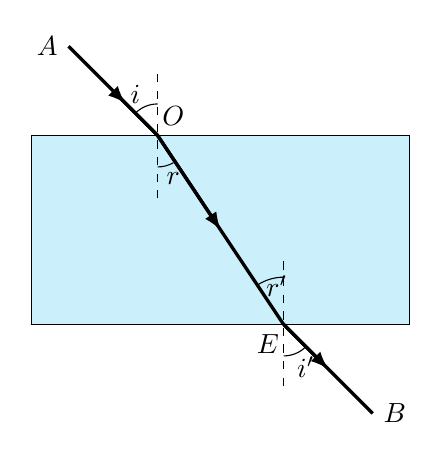
\begin{tikzpicture}[>=latex, scale=.8]
\draw [fill=cyan!20] (-3,-3) rectangle (3,0);
\draw [very thick](-1,0)--(1,-3);	
\node at (-.75,0)[above]{$O$};
\node at (.75,-3)[below]{$E$};
\draw[->, very thick](-1,0)--(0,-1.5)	;
\draw[very thick] (-1,0)--+(135:2)node [left]{$A$};
\draw[very thick] (1,-3)--+(-45:2)node [right]{$B$};
\draw[very thick, -<] (-1,0)--+(135:1);
\draw[very thick, ->] (1,-3)--+(-45:1);
	\draw[dashed] (-1,-1)--(-1,1);
	\draw[dashed] (1,-2)--(1,-4);
\draw (-1,0.5) arc (90:135:.5)node[above]{$i$};
\draw (1,-3.5) arc (-90:-45:.5)node[below]{$i'$};
\draw (-1,-0.5) arc (-90:-60:.5)node[below]{$r$};
\draw (1,-2.25) arc (90:125:.75)node[right]{$r'$};


	\end{tikzpicture}
	\caption{}
\end{figure}


\begin{solution}
    光线以入射角$i$射在玻璃砖的上表面上,经玻璃砖折射
后从下表射出的光路图如图5.21所示。设光从空气进入
玻璃砖上表面后的折射角为$r$,射到下表面的入射角为$r'$,从
下表面进入空气后的折射角为$i'$,玻璃的折射率为$n$。根据
光的折射定律,
在上表面处
\[\frac{\sin i}{\sin r}=n \]
即
\begin{equation}
    \sin i=n\sin r 
\end{equation}
在下表面处
\[\frac{\sin r'}{\sin i'}=\frac{1}{n} \]
即
\begin{equation}
    \sin i' =n \sin r'
\end{equation}

由于上下两表面平行,所以
\[r'=r,\qquad \sin r'=\sin r \]
由(5.1)
(5.2)两式可得
\[\begin{split}
    \sin i'&=\sin i\\
i'&=i    
\end{split}\]

可见,从玻璃砖下表面射出的光线$EB$平行于射到上表面
的入射光线$AO$。
\end{solution}


这个例题告诉我们,光线通过两面平行的玻璃板后,传播
方向不变,但是从图中可以看出,射出的光线跟入射光线相
比,侧移了一段距离。计算表明,玻璃板越薄,光线侧移的距
离越小。

\subsection*{练习四}
\begin{enumerate}
    \item 光线以45$^\circ$的入射角从空气射入折射率为1.55的玻
璃中,折射角是多大?
\item 光线从空气射入水中,要想使折射角等于30$^\circ$,入射
角应为多大?
\item 根据水和岩盐的折射率,分别算出它们中的光速,水
中的光速大约是真空中光速的几分之几?
\item 图5.22是光线由空气进入某种媒质时的折射情况。
试由图中所给的数据求出这种媒质的折射率和这种媒质中的
光速。
\begin{figure}[htp]
	\centering
	\begin{tikzpicture}[>=latex]
\fill [cyan!20] (-3,-2) rectangle (3,0);
\node at (1,1){空气};
	\draw[dashed] (0,-1)--(0,1);
\draw(-3,0)--(3,0);
\draw[->, very thick] (0,0)--(-55:1.5); \draw[very thick] (0,0)--(-55:2);
\draw[->, very thick] (150:3)--(150:1.5); \draw[very thick] (0,0)--(150:3);
\draw (.5,0) arc (0:-55:.5) node [right] {$55^\circ$};
\draw (-1,0) arc (180:150:1) node [below] {$30^\circ$};

	\end{tikzpicture}
	\caption{}
\end{figure}

    \item 根据上节表中给出的折射率填空:
    \begin{enumerate}
        \item 光线从水中垂直射入空气中时,折射角\underline{\qquad}
    于入射
    角;从玻璃斜射入水中时,折射角\underline{\qquad}于入射角;从空气斜射
    入酒精中时,折射角\underline{\qquad}
    于入射角;从岩盐斜射入水晶中时,
    折射角\underline{\qquad}
    于入射角。
    \item 二硫化碳比水的折射率大,由此可知二硫化碳中的光
    速比水中的光速\underline{\qquad};二者相比,二硫化碳是光\underline{\qquad}
    媒质,水是光\underline{\qquad}
    媒质。
    \end{enumerate}
    
    \item 你在池边沿斜线向水面下看去,看到水中有一条鱼,
    你所看到的鱼的位置比实际的深还是浅?如果鱼也看到了你,
    鱼所看到的你的头的位置比实际的高还是低?
    \item 把一块厚玻璃板压在书上,透过玻璃板看书上的字
    跟拿走玻璃板直接看,感觉有什么不同?做做看,并解释看到
    的现象。
\end{enumerate}

\section{全反射}
\subsection{全反射现象}

光从光密媒质射入光疏媒质时,折射角大
于入射角。由此可以预料,当入射角增大到某一角度时,折射
角将等于90$^\circ$,入射角再增大,就不再有折射光线了。
    \begin{figure}[htp]
        \centering
        \begin{tikzpicture}[>=latex]
    \draw [fill=cyan!20] (-2,0) arc (180:360:2);
    
    \draw[->, very thick] (0,0)--(20:1.5); \draw[very thick] (0,0)--(20:3)node[above]{折射光线};
    \draw[->, very thick]  (0,0)--(-45:1.5); \draw[very thick]  (0,0)--(-45:3)node[below]{反射光线};
        \draw[very thick] (0,0)--(225:3);	\draw [<-,very thick](225:1.5)--(225:3);	
    \node at (-1,1){空气};
        \draw (-2,0)--(2,0);
    \draw[dashed] (0,-1)--(0,1);
    \node at (225:3.25){\Sun};
    \node at (225:3.5)[below]{光源};
        \end{tikzpicture}
        \caption{观察全反射现象}
    \end{figure}

上述现象可以用图5.23所示的半圆形玻璃砖来观察。让
光线沿着半圆形玻璃砖的半径射到直边上,可以看到,一部分
光线从直边折射到空气中,一部分光线反射回玻璃。逐渐增
大光线的入射角,将会看到,折射光线离法线越来越远,而且
折射光线越来越弱,反射光线越来越强,当入射角增大到某
一角度时,折射光线消失,只剩下反射光线,光全部反射回玻
璃中,这种现象叫做\textbf{全反射}。

\subsection{临界角}

折射角等于90$^\circ$时的入射角叫做\textbf{临界角}。光线
从光密媒质射入光疏媒质,当入射角大于临界角时,就发生全
反射现象。

利用光的折射定律,可以求出各种媒质对空气(或真空)
的临界角。如果用$C$表示临界角,$n$表示媒质的折射率,那么,
由于空气对该媒质的折射率等于$1/n$,
所以
\[\frac{\sin C}{\sin 90^\circ}=\frac{1}{n} \]
由此可得
\[\sin C=\frac{1}{n} \]

因此,已知媒质的折射率,利用上式就可以求出这种媒质
对空气(或真空)的临界角。

光的全反射现象在自然界中经常可以看到。水或玻璃巾
的气泡看起来特别明亮,就是因为光从水或玻璃射向气泡时,
在界面发生全反射。露水珠或喷泉的水珠,在阳光照耀下格
外明亮,也是因为射进水珠的光在水珠内发生全反射。

\subsection{光导纤维}
\begin{figure}[htp]\centering
    \includegraphics[scale=.6]{fig/5-24.png}
    \caption{弯曲的玻璃棒能传输光}
    \end{figure}

光从玻璃射入空气时,如果入射角大于临界
角,就发生全反射,使光不能从玻璃射到空气中。这一现象使
人们受到启发,试图用玻璃棒来传输光。如图5.24所示,把
一根弯曲的玻璃棒插在暗盒的一边,打开盒里的电灯,可以看
到从玻璃棒的下端有明亮的光传出来,如果照在纸上,就出现
一个明亮的光斑,这是因为从玻璃捧上端进入棒内的光线,
在棒的内壁上发生全反射;经过多次全反射,光线最后从棒的
下端传出来。
\begin{figure}[htp]\centering
    \includegraphics[scale=1]{fig/5-25.pdf}
    \caption{光导纤维}
    \end{figure}

现代科学技术中用的光导纤维,就是利用上述现象制成
的,光导纤维简称光纤,是一种比头发还细的玻璃丝,这种
玻璃丝分为内外两层(芯线和包层),芯线的折射率比包层的
折射率大,光从芯线射向包层时能发生全反射,这样光就在芯
线内从光纤的一端传输到另一端(图5.25)。
\begin{figure}[htp]\centering
    \includegraphics[scale=1]{fig/5-26.pdf}
    \caption{光导纤维传像}
    \end{figure}

如果把许多光纤并成束,并使束中各条光纤的相对位
置保持不变,就可以用来传递图像(图5.26)。医学上用光纤
来观察人体内脏的内窥镜,例如胃镜,就是用这个道理制
作的。

光导纤维在现代科学技术中有重要的应用,就象无线电
技术中把信号调制到无线电波上一样,把要传送的信号调制
到光波上,让光载着信号沿光导纤维传送出去,就可以实现光
纤通讯。光纤通讯能够同时传送大量信号,对信息的传输能
力很大,这是它的突出优点。采用光纤通讯将会引起通讯技
术的重大变革,光纤通讯在一些先进国家正在进入实用阶
段。我国也在努力提高光纤技术的水平,积极进行光纤通讯
试验,以适应现代科学技术革命的需要,这方面有许多工作
等待人们去做。

\section*{阅读材料:海市蜃楼}

夏天,在平静无风的海面上,向远方望去,有时能看到山
峰、船舶、楼台、亭阁、集市、庙宇等出现在远方的空中,古人
不明白产生这种景象的原因,对它作了不科学的解释,认为是
海中蛟龙(即蜃)吐出的气结成的,因而叫做“海市蜃楼”.1981
年8月19日文汇报曾以《蓬莱阁上观胜景,庙岛海面出蜃楼》
为题,登载了这年7月10日下午在山东省蓬莱市海面上出现
海市蜃楼的消息,当时有四、五百游人观赏了这一奇异景象。

海市蜃楼是光在密度分布不均匀的空气中传播时发生全
反射而产生的,夏天,海面上的下层空气,温度比上层低,密度
比上层大,折射率也比上层大。我们可以把海面上的空气看
作是由折射率不同的许多层气体组成的,远处的山峰、船舶、
楼房、人等反射出来的光线射向空中时,由于不断被折射,越
来越偏离法线方向,进入上层空气的入射角不断增大,以致发
生全反射,光线反射回地面,人们逆着光线看去,就会看到远
方的景物悬在空中(图5.27)。
\begin{figure}[htp]\centering
    \includegraphics[scale=.6]{fig/5-27.png}
    \caption{海市蜃楼}
    \end{figure}

在沙漠里也会看到海市蜃楼现象,太阳照到沙地上,接
近沙面的热空气层比上层空气的密度小,折射率也小。从远
处物体射向地面的光线,进入折射率小的热空气层时被折射,
入射角逐渐增大,也可能发生全反射,人们逆着反射光线看
去,就会看到远处物体的倒影(图5.28),仿佛是从水面反射出
来的一样,沙漠里的行人常被这种景象所迷惑,以为前方有
水源而奔向前去,但总是可望而不可及。
\begin{figure}[htp]\centering
    \includegraphics[scale=.6]{fig/5-28.png}
    \caption{沙漠里的海市蜃楼}
    \end{figure}

在炎热夏天的柏油马路上,有时也能看到上述现象。光
线被贴近路面的热空气全反射,从远处看去,路面显得格外明
亮光滑,就象用水淋过一样。

\subsection*{练习五}

\begin{enumerate}
    \item 水和金刚石的临界角各是多大?
    \item 图5.29表示一个横
截面为等腰直角三角形的玻璃
棱镜。当光从它的一个直角边垂直射入时,就从另一个直角
边垂直射出来,而没有光从斜
边射出,这种棱镜可以使光的
传播方向改变90$^\circ$。说明它的
道理。
\begin{figure}[htp]
	\centering
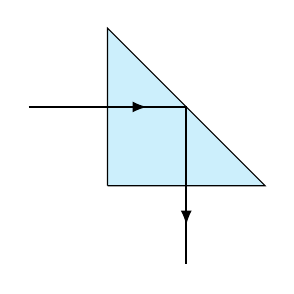
\begin{tikzpicture}[>=latex]
  \draw [fill=cyan!20](0,0)--(2,0)--(0,2)--(0,0);
    \draw[ thick] (-1,1)--(1,1)--(1,-1);
\draw[->,  thick](-1,1)--(.5,1); \draw[->,  thick](1,1)--(1,-.5); 
\end{tikzpicture}
	\caption{}
\end{figure}

\item 光线从空气射入水中时,光线在水中的折射角最大为多少度?
\item 潜水的人在水面下能看到水面上的全部景象,因为
水面上180$^\circ$范围内射入水中的光线全部集中在水下97.5$^\circ$的视野内(图5.30),试说明它的道理。
\begin{figure}[htp]\centering
    \includegraphics[scale=.6]{fig/5-30.png}
    \caption{}
    \end{figure}
\end{enumerate}

\section{棱镜}

光学仪器中常用的棱镜是横截面为三角形的三棱镜,通
常简称为棱镜,下面我们来研究棱镜对光的作用。

\subsection{通过棱镜的光线~~色散}

让一束单色光从空气射向玻璃
棱镜的一个侧面,可以看到,光线通过棱镜,从另一个侧面射
出来时,方向发生了明显的变化;光线向棱镜的底面偏折(图
5.31),这是因为光线在棱镜的两个侧面上发生折射时,两次
向底面偏折所造成的。偏折角度$\theta$跟棱镜材料的折射率有
关\footnote{偏折角度$\theta$还跟入射角的大小有关系,这个问题高中不讨论。},折射率越大,偏折角度越大。
\begin{figure}[htp]\centering
    \includegraphics[scale=1]{fig/5-31.PDF}
    \caption{光线通过棱镜后,向底面偏折}
    \end{figure}

让一束白光射向玻璃棱镜,可以看到,白光通过棱镜后,
发生色散,在光屏上形成一条彩色的光带(图5.32),叫做\textbf{光
谱}。红光在最上端,紫光在最下端,中间是橙、黄、绿、蓝等色。
这表明各种色光通过棱镜后的偏折角度不同。红光的偏折角
度最小,紫光的偏折角度最大。
\begin{figure}[htp]\centering
    \includegraphics[scale=1.2]{fig/5-32.pdf}
    \caption{棱镜使白光发生色散}
    \end{figure}

    不同色光通过棱镜后的偏折角度不同,表明棱镜材料对
    不同色光的折射率不同,红光的偏折角度小,表示棱镜材料对
    红光的折射率小;紫光的偏折角度大,表示棱镜材料对紫光的
    折射率大,下表是实验测得的冕牌玻璃对各种色光的折
    射率。

\begin{center}
    \begin{tabular}{ccccccc}
        \hline
        色光&        紫&        蓝&        绿&        黄&        橙&        红\\
        \hline
        折射率&        1.532&        1.528&        1.519&        1.517&        1.514&        1.513\\
        \hline
    \end{tabular}
\end{center}

我们知道,媒质的折射率等于光在真空中的速度跟在这
种媒质中的速度之比。各种色光在真空中的速度是一样的,
都等于$c$,它们在同一媒质(例如玻璃)中的折射率不同,表明
它们在同一媒质中的速度不同,红光的折射率比其他色光小,
表明红光在媒质中的速度比其他色光大。

\subsection{全反射棱镜}

从练习五的第2题知道,横截面为等腰直
角三角形的玻璃棱镜对光能起全反射作用,这种棱镜叫做\textbf{全
反射棱镜}。

通常用的反光镜背面都镀有一层银膜,靠这层银膜来反
射光。这种镀膜的反光镜不能
使光全部反射,大约有10\%的
光被吸收掉。全反射棱镜能够
把入射光全部反射出去,所以
在一些精密的光学仪器中都
用全反射棱镜代替镀膜的平面
镜,例如,潜水艇的潜望镜中就
使用全反射棱镜(图5.33)。
\begin{figure}[htp]
	\centering
	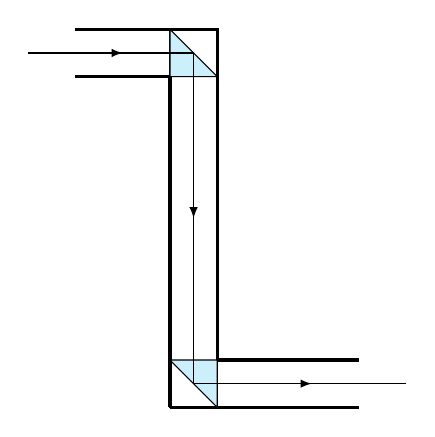
\begin{tikzpicture}[>=latex, scale=1.2]
	\draw (0,0) rectangle (.5, 4);
	\draw [very thick](0,0)--(2,0);  \draw [very thick](.5,0.5)--(2,0.5);
\draw [very thick](0,0)--(0,3.5)--(-1,3.5);  \draw [very thick](.5,0.5)--(.5,4)--(-1,4);
	%\draw (0,4)--(-2,4);  \draw (0,3.5)--(-2,3.5);
\draw [fill=cyan!20](0,0.5)--(.5,.5)--(.5,0)--(0,0.5);
\draw [fill=cyan!20](0,4)--(0,3.5)--(.5,3.5)--(0,4);

\draw(-1.5,3.75)--(.25,3.75)--(0.25,.25)--(2.5,.25);
\draw[->](-1,3.75)--(-.5,3.75);
\draw[->](.25,3.75)--(.25,2);
\draw[->](0.25,.25)--(1.5,.25);
	\end{tikzpicture}
	\caption{潜望镜中的全反射棱镜}
\end{figure}


\subsection*{练习六}
\begin{enumerate}
    \item 说明图5.31中,光线通过棱镜的$AB$和$AC$两个侧
面时,为什么都向底面偏折,如果这个棱镜的里面是空气,周
围是水,当光线通过这个空气棱镜时,射出的光线是否还向底
面偏折?画出这种情况下的光路图来。
\item 冕牌玻璃对紫光的折射率为1.532,对红光的折射率
为1.513。紫光和红光在这种玻璃中的速度各是多大?
\item 什么形状的全反射棱镜可以使光线改变180$^\circ$?这时
光线应从哪边射入?画出光路图来。
\item 光线通过棱镜时,偏折角度$\theta$跟棱镜材料的折射率
有关。设图5.31中光线对棱镜的侧面$AB$的入射角以及棱
镜的顶角$A$的大小保持不变。试定性地讨论:棱镜材料的折
射率越大,偏折角度也越大。
\end{enumerate}

\section{透镜}
折射面是两个球面,或者一个是球面,另一个是平面的透
明体,叫做透镜。透镜通常是用玻璃磨成的,它是光学仪器中
经常使用的基本元件。

\subsection{凸透镜和凹透镜}

透镜可分为两类。一类是中间厚、边缘
薄的,叫做\textbf{凸透镜},凸透镜对光线起会聚作用,又叫做\textbf{会聚透
镜},另一类是中间薄、边缘厚的,叫做\textbf{凹透镜}。凹透镜对光线
起发散作用,又叫做\textbf{发散透镜}。
\begin{figure}[htp]
    \centering
    \begin{minipage}[t]{0.48\textwidth}
    \centering
    \includegraphics[scale=1.2]{fig/5-34-1.pdf}
    \end{minipage}
    \begin{minipage}[t]{0.48\textwidth}
    \centering
    \includegraphics[scale=.8]{fig/5-34-2.pdf}
    \end{minipage}
    \caption{}
    \end{figure}


凸镜为什么能使光线会聚,凹透镜为什么能使光线发
散呢?其原理可用棱镜对光线的偏折作用来说明,如图5.34所示,透镜可以看作是由许多棱镜组成的。凸透镜上部的
棱镜底面朝下,光线通过时都向下偏折;下部的棱镜底面朝
上,光线通过时都向上偏折,因此,凸透镜使光线会聚。与此
相反,凹透镜上部的棱镜底面朝上,光线通过时都向上偏折;
下部的棱镜底面朝下,光线通过时都向下偏折。因此,凹透镜
使光线发散。

\subsection{透镜的主轴、光心和焦点}

透镜的两个球面都有自己的
球心,如图5.35中的$C_1$、$C_2$所示,我们把通过两球心$C_1$、$C_2$
的直线,叫做透镜的\textbf{主光轴},简称主轴。通常把厚度比球面的
半径小得多的透镜,叫做薄透镜。我们在后面讨论的都是薄
透镜。
\begin{figure}[htp]\centering
\begin{tikzpicture}[>=latex, scale=.6]
\draw [dashed](-3.5,0)--(5,0);
\draw (-1,0) circle (1.5);
\draw (1.6,0) circle(2);
\node at (-1,0)[above]{$C_1$};
\node at (1.6,0)[above]{$C_2$};
\node at (-0.05,0)[below]{$O$};
\draw [fill=black] (-1,0) circle (1.5pt);
\draw [fill=black] (1.6,0) circle (1.5pt);
\draw [fill=black] (-0.05,0) circle (1.5pt);
\draw [pattern=north east lines](-0.05,1.15) to [bend right=32] (-0.05,-1.15) to [bend right=54](-0.05,1.15);
\end{tikzpicture}
\begin{tikzpicture}[>=latex, scale=.6]
    \draw [dashed](-3,0)--(7,0);
    \draw (-1,0) circle (2);
    \draw (3.6,0) circle(2);
    \node at (-1,0)[above]{$C_1$};
    \node at (3.6,0)[above]{$C_2$};
    \node at (1.3,0)[below]{$O$};
    \draw [fill=black] (-1,0) circle (1.5pt);
    \draw [fill=black] (3.6,0) circle (1.5pt);
    \draw [fill=black] (1.3,0) circle (1.5pt);
    \draw [pattern=north east lines](.65,1.15) to [bend left=32] (.65,-1.15) --(1.95,-1.15) to [bend left=32](1.95,1.15)--(.65,1.15);

\end{tikzpicture}
    \caption{透镜的主轴}
    \end{figure}

主轴跟透镜的两面各有一个交点,对于薄透镜来说,这两
个交点可以看作是重合在一起的,这一点叫做透镜的\textbf{光心},用
$O$表示。透镜的中央部分相当于两面平行的薄玻璃板,通过
光心的光线相当于通过这个薄玻璃板,因此,不管从任何方向
通过光心的光线,传播方向都不改变,这是光心的重要性质。

平行于主轴的光线,通过凸透镜后会聚于主轴上的一点
(图5.36甲$F'$),这个点叫做\textbf{凸透镜的焦点}。平行于主轴的
光线通过凹透镜后变得发散(图5.36乙),这些发散光线看起
来好象是从它们的反向延长线的交点$F'$发出来的,点$F'$也
在主轴上,叫做\textbf{凹透镜的焦点}。凸透镜的焦点是实焦点,凹透
镜的焦点是虚焦点。
\begin{figure}[htp]\centering
\begin{minipage}[t]{0.48\textwidth}
\centering
\begin{tikzpicture}[>=latex, scale=1]
    \draw [pattern=north east lines] (0,1.2) to [bend left=15] (0,-1.2) to [bend left=15](0,1.2);
    \draw [dashed] (-2.5,0)--(3.2,0);
    \draw (0,0)[fill=black] circle (1.5pt);
    \draw (-2,0)[fill=black] circle (1.5pt);    \draw (2,0)[fill=black] circle (1.5pt);
    \foreach \x in {-.8,-.4,.4,.8}
    {
        \draw[->] (-2.5,\x)--(-2,\x);
    }    

\draw[->] (-2,-.8)--(0,-.8)--(2,0)--(3, .4)   ;
\draw[->] (-2,-.4)--(0,-.4)--(2,0)--(3, .2)   ;
\draw[->] (-2,.4)--(0,.4)--(2,0)--(3, -.2)   ;
\draw[->] (-2,.8)--(0,.8)--(2,0)--(3, -.4)   ;

\node at (-2,0)[above]{$F$};
\node at (2,0)[above]{$F'$};
\node at (-.5,0)[above]{$O$};


\end{tikzpicture}
\caption*{甲}
\end{minipage}
\begin{minipage}[t]{0.48\textwidth}
\centering
\begin{tikzpicture}[>=latex]
    \draw [pattern=north east lines] (0,1.2) to [bend left=15] (0,-1.2)--(.5,-1.2) to [bend left=15](.5,1.2)--(0,1.2);
    \draw [dashed] (-2.5,0)--(3.2,0);
\node at (-2,0) [above]{$F'$};
\node at (2,0) [above]{$F$};
\draw (-2,0)[fill=black] circle (1.5pt);    \draw (2,0)[fill=black] circle (1.5pt);

\foreach \x in {-.8,-.4,.4,.8}
    {
        \draw[->] (-2.5,\x)--(-2,\x);
        \draw[dashed](-2,0)--(0.25,\x);
        \draw[->](0.25,\x)--(2.5,2*\x);
    }  
    \draw  (-2,-.8)--(0.25,-.8)    ;
    \draw  (-2,-.4)--(0.25,-.4)    ;
    \draw  (-2,.4)--(0.25,.4)    ;
    \draw  (-2,.8)--(0.25,.8)    ;
    \draw[->](0.25,0)--(2.5,0);
   \node at (0,0)[above] {$O$};
   \draw (0.25,0)[fill=black] circle (1.5pt); 
\end{tikzpicture}
\caption*{乙}
\end{minipage}
    \caption{}
    \end{figure}

从透镜的焦点到光心的距离,叫做透镜的\textbf{焦距},用$f$表
示。透镜的两侧各有一个焦点,只要透镜两侧的媒质相同,两
个焦点对光心是对称的,两个焦距相等,后面讨论的都是这
种情况。

\subsection*{练习七}
\begin{enumerate}
    \item 有一个不知焦距的凸透镜,用什么办法可以粗略地测出它的焦距?
    \item 利用点光源和凸透镜如何能得到平行光线?
    \item 在图5.37中,画出光线通过透镜后的传播方向。
\end{enumerate}

\begin{figure}\centering
\begin{tikzpicture}[>=latex]
    \draw [pattern=north east lines] (0,1.2) to [bend left=15] (0,-1.2) to [bend left=15](0,1.2);
    \draw [dashed] (-2,0)--(2,0);
\node at (-1.5,0)[below] {$F$};\node at (1.5,0)[below] {$F'$};
\draw (-1.5,0) [fill=black]circle(1.5pt); \draw (1.5,0) [fill=black]circle(1.5pt);
\draw [->](-2,-.7)--(-1.5, -.7);
\draw (-1.5,-.7)--(0, -.7);


\end{tikzpicture}
\begin{tikzpicture}[>=latex]
    \draw [pattern=north east lines] (0,1.2) to [bend left=15] (0,-1.2) to [bend left=15](0,1.2);
    \draw [dashed] (-2,0)--(2,0);
    \node at (-1.5,0)[below] {$F$};\node at (1.5,0)[below] {$F'$};
    \draw (-1.5,0) [fill=black]circle (1.5pt); \draw (1.5,0) [fill=black]circle(1.5pt);
    \draw (-1.5,0)--(0, .7);
    \draw [->](-2,-.7/3)--(-1.5,0);
\end{tikzpicture}


    \begin{tikzpicture}[>=latex]
        \draw [pattern=north east lines] (0,1.2) to [bend left=15] (0,-1.2)--(.5,-1.2) to [bend left=15](.5,1.2)--(0,1.2);
        \node at (-1.5,0)[below] {$F$};\node at (1.5,0)[below] {$F'$};
        \draw (-1.5,0) [fill=black]circle (1.5pt); \draw (1.5,0) [fill=black]circle(1.5pt);
        \draw [dashed] (-2,0)--(2,0);
        \draw [->](-2,.7)--(-1.5, .7);
        \draw (-1.5,.7)--(0.25, .7);
    \end{tikzpicture}
    \begin{tikzpicture}[>=latex]
        \draw [pattern=north east lines] (0,1.2) to [bend left=15] (0,-1.2)--(.5,-1.2) to [bend left=15](.5,1.2)--(0,1.2);
        \node at (-1.5,0)[below] {$F$};\node at (1.5,0)[below] {$F'$};
        \draw (-1.5,0) [fill=black]circle (1.5pt); \draw (1.5,0) [fill=black]circle(1.5pt);
        \draw [dashed] (-2,0)--(2,0);
        \draw [->](-2,.7)--(-1.75/2, .7/2);
        \draw (-1.75/2, .7/2)--(0.25, 0);

    \end{tikzpicture}
    \begin{tikzpicture}[>=latex]
        \draw [pattern=north east lines] (0,1.2) to [bend left=15] (0,-1.2)--(.5,-1.2) to [bend left=15](.5,1.2)--(0,1.2);
        \node at (-1.5,0)[below] {$F$};\node at (1.5,0)[below] {$F'$};
        \draw (-1.5,0) [fill=black]circle (1.5pt); \draw (1.5,0) [fill=black]circle(1.5pt);
\draw [dashed] (-2,0)--(2,0);
\draw[dashed](.25,.5)--(1.5,0);
\draw (-1,1)--(.25,.5);
\draw[->] (-1.625,1.25)--(-1,1);
    \end{tikzpicture}
\caption{}
\end{figure}

 \section{透镜成像}
    利用透镜可以使物体成像,这是透镜的一个重要应用,透
    镜所成的像跟物体离透镜的距离有关系,下面我们用实验来
    研究透镜成像的情况。

    象图5.38那样,把蜡烛和光屏放在光具座的两端,把焦
    距已知的凸透镜放在蜡烛和光屏之间。调整凸透镜和光屏的
    高度,使烛焰的中点、凸透镜的光心、光屏的中点一样高,以使
    烛焰的像能成在光屏上。
    \begin{figure}[htp]\centering
        \includegraphics[scale=.6]{fig/5-38.png}
        \caption{研究透镜成像}
        \end{figure}

    先使蜡烛到透镜的距离——物距$u$大于2倍焦距($u>
    2f$),移动光屏,直到在屏上出现清晰的蜡烛的像。可以看到,
    这个像是缩小、倒立的,这时光屏到凸透镜的距离——像距
    小于2倍焦距$2f$。这个像是蜡烛发出的光通过凸透镜后会
    聚而成的,是实像。

    缩短蜡烛到凸透镜的距离,移动光屏,使像仍成在光屏
    上。可以看到,像变大。当物距等于2倍焦距时,像的大小跟
    蜡烛相同,这时像距也等于2倍焦距.

    继续缩短蜡烛到凸透镜的距离,使$2f>u>f$。可以看到,
    这时所成的像大于蜡烛,像距$v>2f$。如果再缩短物距,使$u=
    f$,则无论怎样移动光屏,也得不到像了。

    进一步减小物距,使$u<f$,光屏上仍得不到蜡烛的像。但
    是,如果从光屏这边朝着透镜看去,可以看到一个正立、放大
    的像,与蜡烛位于凸透镜的同侧,这个像是由通过凸透镜的
    光线的反向延长线会聚成的,是虚像。

    总结以上凸透镜成像的情况,可以看出:当$u>2f$时,成
    倒立、缩小的实像;当$u=2f$时,所成的倒立的实像跟物体大
    小相等;当$2f>u>f$时,成倒立、放大的实像;当$u<f$时,成
    正立、放大的虚像。

    改用凹透镜来做上面的实验,可以看到,无论怎样改变
    蜡烛到凹透镜的距离$u$,在光屏上都得不到蜡烛的实像,而
    只能通过凹透镜看到一个与蜡烛位于同侧的正立、缩小的
    虚像。

    \subsection*{练习八}
    \begin{enumerate}
        \item 放大镜所成的像是正立、放大的,这是实像还是虚
    像?放大镜应该是什么透镜?如果其焦距为$f$,镜到物的距离
    最大不能超过多少?
    \item 幻灯机所成的像是什么像?它的镜头应该是什么透
    镜?如果镜头的焦距为8厘米,镜头到幻灯片的距离只能在什
    么范围内变化?
    \item 照相机所成的像是什么像?它的镜头应该是什么透
    镜?如果镜头的焦距为7.5厘米,镜头到底片的距离最短不能
    小于多少?
    \end{enumerate}

    \section{透镜成像作图法}
    物体通过透镜所成的像,可以用作图方法求出。我们知
    道,发光点S通过凸透镜所成的实像$S'$,是从$S$射向凸透镜的
    所有光线经凸透镜折射后的会聚点(图5.39)。所以我们只要
    找出其中两条光线的会聚点,就可以确定像的位置。
    \begin{figure}[htp]\centering
    \begin{tikzpicture}[>=latex, scale=.8]
    \draw [pattern=north east lines] (0,2) to [bend left=20] (0,-2) to [bend left=20](0,2);
    \draw [dashdotted] (-5,0)--(5,0);
    \node at (0,0)[fill=white, above]{$O$};
    \draw[thick] (-4,1.5)node[left]{$S$}--(0,1.5)--(2,0)--(4,-1.5)node[right]{$S'$};
    \draw[thick] (-4,1.5) --(0,-1.5)--(4,-1.5);
    \draw[thick] (-4,1.5)--(0,.5)--(4,-1.5);
    \draw[thick] (-4,1.5)--(0,-.5)--(4,-1.5);
    \node at (2,0)[above]{$F'$};
    \node at (-2,0)[below]{$F$};
    \draw (-4,1.5) [fill=black] circle (1.5pt);
    \draw (4,-1.5) [fill=black] circle (1.5pt);
    \draw (0,0) [fill=black] circle (1.5pt);
    \draw (-2,0) [fill=black] circle (1.5pt);
    \draw (2,0) [fill=black] circle (1.5pt);
    
    \draw [->](-3,1.5)--(-1,1.5);
    \draw [->](1,-1.5)--(3,-1.5);
    \draw [->](-2,0)--(-1,-1.5/2);
    \draw [->](2,0)--(3,-1.5/2);

    \draw [->](0,.5)--(2,-.5);
    \draw [>-](-2,1 )--(0,.5);
    \draw [->](0,-.5)--(2,-1);
    \draw [>-](-2,.5 )--(0,-.5);    
    
    \end{tikzpicture}
        \caption{像是通过凸透镜的所有光线的会聚点}
        \end{figure}
 
    
    当发光点不在主轴上时,它射向凸透镜的光线中,下列三
    条光线通过凸透镜后的折射光线的方向很容易确定:
    \begin{enumerate}
        \item   跟主轴平行的光线,折射后通过焦点;
        \item 通过焦点的光线,折射后跟主轴平行;
        \item 通过光心的光线经过透镜后方向不变。
    \end{enumerate}

    应用这三条光线中的任意两条,就可以求出发光点$S$的
    像$S'$(图5.40)。
    \begin{figure}[htp]\centering
\begin{tikzpicture}[>=latex,scale=.8]
\draw [pattern=north east lines] (0,2) to [bend left=20] (0,-2) to [bend left=20](0,2);
\node at (0,0)[fill=white, above]{$O$};
\draw [dashdotted] (-5,0)--(5,0);
\draw[thick] (-4,1.5)node[left]{$S$}--(0,1.5)--(2,0)--(4,-1.5)node[right]{$S'$};
\draw[thick] (-4,1.5) --(0,-1.5)--(4,-1.5);
\draw[thick] (-4,1.5)--(4,-1.5);
\node at (2,0)[above]{$F'$};
\node at (-2,0)[below]{$F$};
\draw (-4,1.5) [fill=black] circle (1.5pt);
\draw (4,-1.5) [fill=black] circle (1.5pt);
\draw (0,0) [fill=black] circle (1.5pt);
\draw (-2,0) [fill=black] circle (1.5pt);
\draw (2,0) [fill=black] circle (1.5pt);

\draw [->](-3,1.5)--(-1,1.5);
\draw [->](1,-1.5)--(3,-1.5);
\draw [->](-2,0)--(-1,-1.5/2);
\draw [->](2,0)--(3,-1.5/2);
\draw [->](0,0)--(2,-1.5/2);
\draw [>-](-2,1.5/2)--(0,0);


\end{tikzpicture}
        \caption{}
        \end{figure}

    一个物体可以看作是由许多点组成的,每个点发出的光
    线经过透镜后都形成一个像点,所有的像点合在一起就是整
    个物体的像。实际作图时,只要求出物体上下两个端点的像,
    就可以求出物体的像,因为物体上其他各点的像都在这两个
    像点之间。

    作图中,通常用一根两端带箭头的直线表示透镜,跟它垂
    直的直线表示主轴,交点$O$表示光心(图5.41)。
    \begin{figure}[htp]\centering
\begin{circuitikz}
\draw[<->, very thick ] (0,1.2)--(0,-1.2);
\draw [dashed](-1,0)--(1,0);
\node at (-.2,-.2){$O$};
\node at (0,-1.5){甲};
\end{circuitikz}
\qquad 
\begin{circuitikz}
\draw[>-<, very thick ] (0,1.2)--(0,-1.2);
\draw [dashed](-1,0)--(1,0);
\node at (-.2,-.2){$O$};
\node at (0,-1.5){乙};
\end{circuitikz}
        \caption{透镜的符号\\
        甲:凸透镜;        乙:凹透镜}
        \end{figure}

        图5.42是物体$AB$位于凸透镜二倍焦距以外时用作图法
        求出的像。可以看出,求出的像是倒立、缩小的,像位于二倍
        焦距以内,这跟上节实验中观察到的情况是一致的。物体位于
        二倍焦距处以及位于焦点以外、二倍焦距以内时的成像情况,
        请同学们自己练习用作图法来研究。
        \begin{figure}[htp]\centering
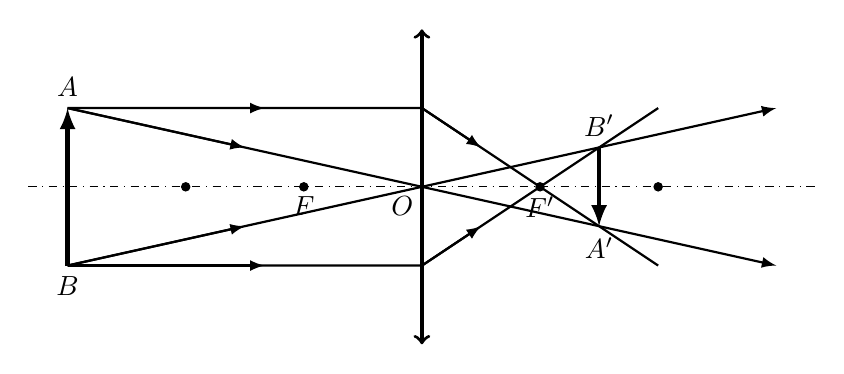
\begin{tikzpicture}[scale=1]
    \draw[<->, very thick ] (0,2)--(0,-2);
\draw[dashdotted](-5,0)--(5,0);
\node at (-1.5,0)[below]{$F$};\node at (1.5,0)[below]{$F'$};\node at (-.25,-.25){$O$};
\draw [fill=black] (-1.5,0) circle (1.5pt);
\draw [fill=black] (1.5,0) circle (1.5pt);
\draw [fill=black] (-3,0) circle (1.5pt);
\draw [fill=black] (3,0) circle (1.5pt);
%\draw [fill=black] (0,0) circle (1.5pt);
\draw [->, ultra thick, >=latex] (-4.5,-1)node[below]{$B$}--(-4.5,1)node[above]{$A$};
\draw [thick](-4.5,-1)--(0,-1)--(1.5,0)--(3,1);  \draw[thick] (-4.5,1)--(0,1)--(1.5,0)--(3,-1);
\draw[->,thick, >=latex] (-4.5,-1)--(-2,-1);  \draw[->,thick, >=latex] (-4.5,1)--(-2,1);
\draw[->, thick, >=latex] (-4.5,1)--(0,0)--(4.5,-1);
\draw[->, thick, >=latex] (-4.5,-1)--(0,0)--(4.5,1);
\draw [->, ultra thick, >=latex] (4.5/2,1/2)node[above]{$B'$}--(4.5/2,-1/2)node[below]{$A'$};

\draw[->, thick, >=latex] (-4.5,1)--(-4.5/2,0.5);
\draw[->, thick, >=latex] (-4.5,-1)--(-4.5/2,-0.5);
\draw[->, thick, >=latex] (0,1)--(1.5/2,0.5);
\draw[->, thick, >=latex] (0,-1)--(1.5/2,-0.5);

\end{tikzpicture}
            \caption{}
\end{figure}

            物体$AB$位于凸透镜的焦点以内时,各点射向透镜的光线
            通过透镜后呈发散状,不能会聚成实像,但是把这些光线沿反
            方向延长后能够会聚成像,这样求出的是物体的虚像(图5.
            43)。从图上可以看出,凸透镜所成的虚像是正立、放大的,跟
            物体位于透镜的同侧。

            \begin{figure}[htp]\centering
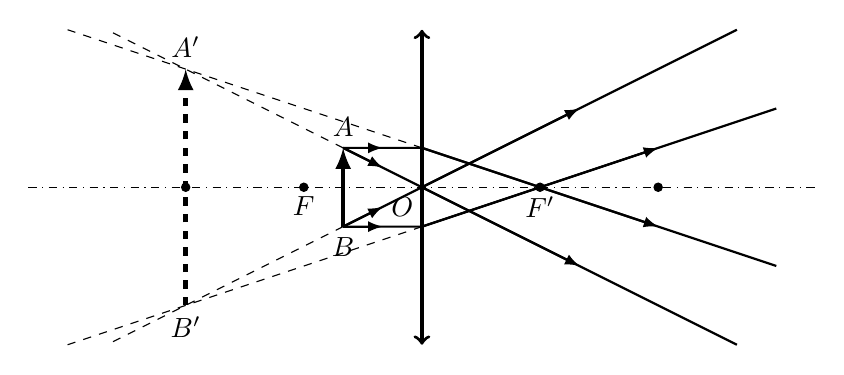
\begin{tikzpicture}
    \draw[<->, very thick ] (0,2)--(0,-2);
    \draw[dashdotted](-5,0)--(5,0);
    \node at (-1.5,0)[below]{$F$};\node at (1.5,0)[below]{$F'$};\node at (-.25,-.25){$O$};
    \draw [thick](-1,.5)--(0,.5)--(1.5,0)--(4.5,-1); 
    \draw [thick](-1,-.5)--(0,-.5)--(1.5,0)--(4.5,1); 
    \draw [thick](-1,.5)--(0,0)--(4,-2);
    \draw [thick](-1,-.5)--(0,0)--(4,2);
    \draw [->, ultra thick, >=latex] (-1,-.5)node[below]{$B$}--(-1,.5)node[above]{$A$};

    \draw[dashed] (0,.5)--(-4.5, 2);   \draw[dashed] (0,-.5)--(-4.5, -2);
    \draw[dashed] (-1,.5)--(-4, 2);   \draw[dashed] (-1,-.5)--(-4, -2);

    \draw [fill=black] (-1.5,0) circle (1.5pt);
    \draw [fill=black] (1.5,0) circle (1.5pt);
    \draw [fill=black] (-3,0) circle (1.5pt);
    \draw [fill=black] (3,0) circle (1.5pt);

    \draw [->, ultra thick, >=latex, dashed] (-3,-1.5)node[below]{$B'$}--(-3,1.5)node[above]{$A'$};


    \draw [->,  thick, >=latex](-1,.5)--(-.5,.5);  \draw [->,  thick, >=latex](0,.5)--(3,-.5);
    \draw [->,  thick, >=latex](-1,-.5)--(-.5,-.5); \draw [->,  thick, >=latex](0,-.5)--(3,.5);
    \draw [->,  thick, >=latex](0,0)--(2,-1);    \draw [->,  thick, >=latex](0,0)--(2,1);

    \draw [->,  thick, >=latex](-1,.5)--(-.5,.25);\draw [->,  thick, >=latex](-1,-.5)--(-.5,-.25);
\end{tikzpicture}
                \caption{}
                \end{figure}

                凹透镜所成的像同样可以用作图法求出。只要注意这时
                平行于主轴的光线,经凹透镜折射后,是折射光线的反向延长
                线通过焦点。图5.44中$A'B'$就是物体$AB$的像。可以看出,
                求出的像与物体位于凹透镜的同侧,是正立、缩小的虚像。

                \begin{figure}[htp]\centering
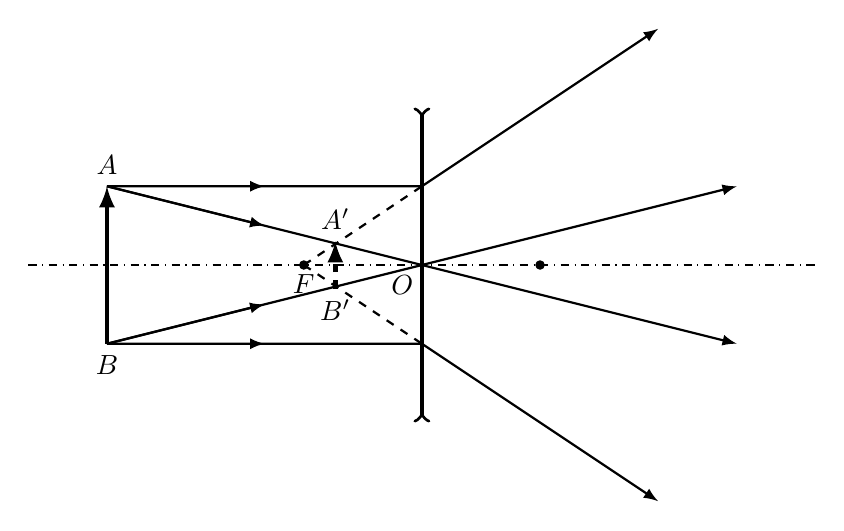
\begin{tikzpicture}
    \draw[>-<, very thick ] (0,2)--(0,-2);
    \draw[dashdotted](-5,0)--(5,0);
    \node at (-1.5,0)[below]{$F$};\node at (-.25,-.25){$O$};
    \draw [fill=black] (-1.5,0) circle (1.5pt);
    \draw [fill=black] (1.5,0) circle (1.5pt);

    \draw [->, ultra thick, >=latex] (-4,-1)node[below]{$B$}--(-4,1)node[above]{$A$};

    \draw [->,  thick, >=latex](-4,1)--(0,1)--(3,3); 
    \draw [->,  thick, >=latex](-4,-1)--(0,-1)--(3,-3); 
    \draw [thick, dashed](-1.5,0)--(0,-1);
    \draw [thick, dashed](-1.5,0)--(0,1);
\draw[->,  thick, >=latex] (-4,1)--(0,0)--(4,-1);
\draw[->,  thick, >=latex] (-4,-1)--(0,0)--(4,1);
\draw[->,  thick, >=latex] (-4,1)--(-2,0.5);
\draw[->,  thick, >=latex] (-4,-1)--(-2,-.5);
\draw [->,  thick, >=latex](-4,1)--(-2,1);
\draw [->,  thick, >=latex](-4,-1)--(-2,-1);
\draw [->, ultra thick, >=latex, dashed ] (-1.1,-.3)node[below]{$B'$}--(-1.1,.3)node[above]{$A'$};



\end{tikzpicture}
                    \caption{}
                    \end{figure}

                    由此可见,用作图法求像时,如果所画光线在通过透镜后
                    相交,得到的就是实像;如果所画光线在通过透镜后的反向延
                    长线相交,得到的就是虚像。


\subsection*{练习九}
\begin{enumerate}
    \item 如图5.45所示,已知物体$AB$通过凸透镜后所成的
    实像$A'B$,试画出从$A$、$B$两点射向凸透镜的任意两条光线
    $AE$、$BD$经过凸透镜折射后的传播方向。
    \begin{figure}[htp]\centering
\begin{tikzpicture}[xscale=1.5]
    \draw[<->, very thick ] (0,2)--(0,-2);
    \draw[dashdotted](-3,0)--(3,0);
\draw[->, ultra thick, >=latex] (-1,0)node[below]{$B$}--(-1,1)node[above]{$A$};

\draw[->,  thick, >=latex] (-1,0)--(0,-.5)node[right]{$D$};
\draw[->,  thick, >=latex] (-1,1)--(0,1.2)node[right]{$E$};
\node at (.25,.25){$O$};
\draw[->, ultra thick, >=latex] (2,0)node[above]{$B'$}--(2,-2)node[below]{$A'$};

\end{tikzpicture}
        \caption{}
        \end{figure}

    \item 一物体位于凸透镜前15厘米,凸透镜的焦距为10厘
米,用作图法求出像到凸透镜的距离。
\item 焦距为10厘米的凹透镜前有一物体,物到镜的距离
为20厘米,用作图法求像到镜的距离。
\item 在图5.46中,$OO'$为透镜的主轴,$A'B'$为物体$AB$
经透镜所成的像。这个透镜是什么透镜?试用作图法求出透
镜和它的焦点的位置。                    
\begin{figure}[htp]\centering
    \begin{tikzpicture}[>=latex]
\draw [dashdotted](0,0)node[left]{$O$}--(7,0)node[right]{$O'$};
\draw [->, very thick](1,0)node[below]{$B$}--(1,1)node[above]{$A$};
\draw [->, very thick](6,0)node[above]{$B'$}--(6,-1.5)node[below]{$A'$};
    \end{tikzpicture}
    \caption{}
    \end{figure}
\end{enumerate}

\section{透镜成像公式}

\subsection{透镜成像公式}

透镜成像的物距、像距和焦距之间的关
系,也可以用公式表示出来,下面我们来推导这个公式。
\begin{figure}[htp]\centering
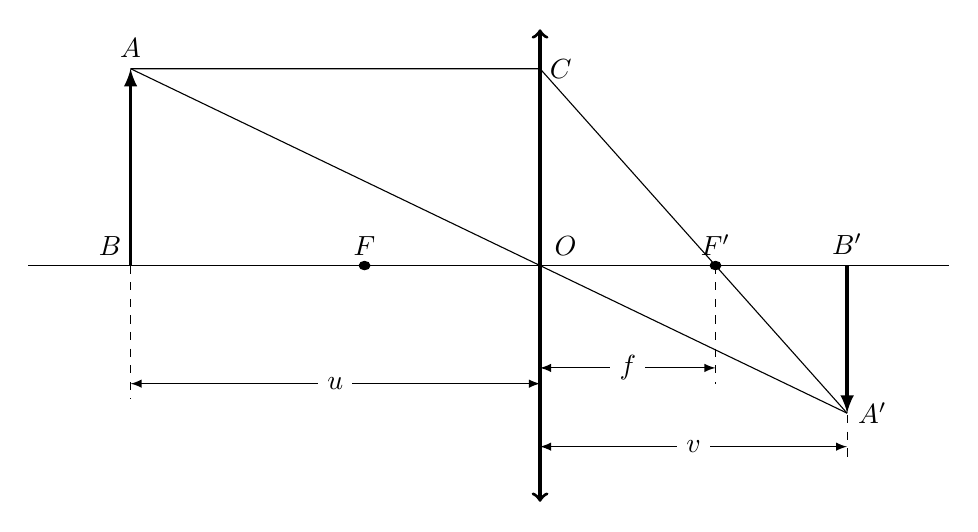
\begin{tikzpicture}[xscale=1.3]
\draw[<->, very thick ] (0,3)--(0,-3);
\draw (-5,0)--(4,0);
\draw [->, very thick, >=latex](-4,0)--(-4,2.5)node[above]{$A$};
\node at (-4-.2,0.25){$B$};
\draw (-4,2.5)--(0,2.5)node[right]{$C$}--(3,-2.5*.75);
\draw (-4,2.5)--(0,0)--(3,-2.5*.75);
\draw [->, very thick, >=latex](3,0)node[above]{$B'$}--(3,-2.5*.75)node[right]{$A'$};
\draw [dashed](12/7,0)node[above]{$F'$}--(12/7,-1.5);
\draw[<->,>=latex] (0,-1.3)--node[fill=white]{$f$}(12/7,-1.3);
\draw[<->,>=latex] (0,-1.5)--node[fill=white]{$u$}(-4,-1.5);
\draw [dashed](-4,0)--(-4,-1.7);  \draw [dashed](3,0)--(3,-2.5);
\draw[<->,>=latex] (0,-2.3)--node[fill=white]{$v$}(3,-2.3);
\node at (0.25,.25){$O$};
\node at (-12/7,.25){$F$};
\draw  (12/7,0)[fill=black] circle (1.5pt);
\draw  (-12/7,0)[fill=black] circle (1.5pt);
\end{tikzpicture}
    \caption{}
    \end{figure}

在图5.47中,$AB$是物体,它到凸透镜的距离为$u$;$A'B'$
是$AB$的像,像到凸透镜的距离为$v$;凸透镜的焦距为$f$。从
图中可以看出,$\triangle COF'  \sim   \triangle A'B'F'$,所以
\[\frac{CO}{A'B'}=\frac{OF'}{B'F'}  \]
另外,$\triangle ABO \sim \triangle A'B'O$,所以
\[\frac{AB}{A'B'}=\frac{BO}{B'O} \]
因为$CO=AB$,所以上面两式的左边相等,因而这两个式子的
右边也相等,即
\[\frac{OF'}{B'F'}=\frac{BO}{B'O} \]
而$OF'=f$,$B'F'=v-f$,$BO=u$,$B'O=v$,把这些代入上式,可
得
\[\frac{f}{v-f}=\frac{u}{v} \]
这个式子用起来不方便,变形后得到
\[fv+fu=uv \]
再用$uvf$除等式两边,就得到凸透镜成像的公式:
\[\frac{1}{u}+\frac{1}{v}=\frac{1}{f}  \]

上面的公式也适用于凹透镜成像(同学们可在后面的练
习中自己证明)。

在运用透镜成像的公式时,需要注意:凸透镜的焦距$f$取
正值,凹透镜的焦距$f$取负值;物体到透镜的距离$u$总取正
值;实像的像距$v$取正值,虚像的像距$v$取负值。

\subsection{像的放大率}

透镜所成的像跟物体相比,可以是放大或
缩小的,也可以跟物体大小相等。为了说明像的放大情况,我
们把像的长度$A'B'$跟物体的长度$AB$之比,叫做\textbf{像的放大率},
并且用$m$表示,即放大率
\[m=\frac{A'B'}{AB} \]

从图5.47可知,
\[\frac{A'B'}{AB}=\frac{v}{u} \]
所以
\[m=\frac{v}{u}\]
即像的放大率等于像距与物距的比值。计算放大率时像距$v$
取绝对值,所以放大率$m$总是正值。

\begin{example}
    下面是一种测量凸透镜焦距的方法:如图5.48
所示,使蜡烛和光屏相距一定的距离$L$,将凸透镜从蜡烛向光屏移动,移动到位置$A$时,在光屏上得到蜡烛放大的实像;移
动到位置$B$时,在光屏上得到蜡烛缩小的实像,测出$A$、$B$间
的距离$d$,利用测得的$L$和$d$即可求出凸透镜的焦距。试求
出这个焦距。
\end{example}

\begin{figure}[htp]
	\centering
\begin{tikzpicture}[>=latex]
  \draw[dash dot](-3,0)--(6,0);
\draw [->, very thick](-2.5,0)--(-2.5,2)node[above]{蜡烛};
\draw [dashed](-2.5,0)--(-2.5, -2);
\draw [dashed](0,1.5)--(0, -.75);
\draw [dashed](3.5,0)--(3.5, -1.5);
\draw [dashed](5.5,0)--(5.5, -2);
\draw [very thick](5.5,0)--(5.5, 3)node[right]{屏};
\draw [<->](-2.5,.75)--node[fill=white]{$u_1$}(0,.75);
\draw [<->](5.5,.75)--node[fill=white]{$v_1$}(0,.75);
\draw [<->](3.5,-.5)--node[fill=white]{$d$}(0,-.5);
\draw [<->](-2.5,-1)--node[fill=white]{$u_2$}(3.5,-1);
    \draw [<->](5.5,-1)--node[fill=white]{$v_2$}(3.5,-1);
\draw [<->](-2.5,-1.5)--node[fill=white]{$L$}(5.5,-1.5);
\fill (0,0) circle (1.5pt);  \fill (3.5,0) circle (1.5pt)node[above]{$B$};
\node at (.2,0)[above]{$A$};
\end{tikzpicture}
	\caption{}
\end{figure}

\begin{solution}
    设凸透镜的焦距为$f$,透镜在$A$时物距为$u_1$,像距为$v_1$,
    透镜在$B$时物距为$u_2$,像距为$v_2$。利用透镜成像公式可得:
   \begin{align}
\frac{1}{u_1}+\frac{1}{v_1}&=\frac{1}{f}\\
\frac{1}{u_2}+\frac{1}{v_2}&=\frac{1}{f}
   \end{align}
 
    由(5.3)(5.4)两式得
\[\frac{1}{u_1}+\frac{1}{v_1}=\frac{1}{u_2}+\frac{1}{v_2} \]
    
从图上可知,$v_1=L-u_1$,$u_2=u_1+d$,$v_2=L-u_1-d$,代入
    上式,以消去$v_1$、$u_2$和$v_2$,得
    \[\frac{1}{u_1}+\frac{1}{L-u_1}=\frac{1}{u_1+d}+\frac{1}{L-u_1-d} \]

    把上式整理化简,可得
\[u_1=\frac{1}{2}(L-d) \]
    把上式和$v_1=L-u_1$代入(5.3)式,化简后可得
\[f=\frac{L^2-d^2}{4L} \]
    这就是所求的计算凸透镜焦距的公式。这个公式在后面测定
    凸透镜焦距的实验中将要用到。
\end{solution}

\subsection*{练习十}

\begin{enumerate}
    \item 试证明:
$\dfrac{1}{u}+\dfrac{1}{v}=\dfrac{1}{f}$也
适用于凹透镜成像。(提示:
对于凹透镜$f$和$v$应取负值)
\item  利用公式
$\dfrac{1}{u}+\dfrac{1}{v}=\dfrac{1}{f}$,
试讨论:
\begin{enumerate}
    \item 对于凸透镜,物距$u$在什么范围内变化时,$v$为正值,
    成实像?在什么范围内变化时,$v$为负值,成虚像?
    \item 对于凹透镜,$v$能否为正值?
\end{enumerate}
\item 一支蜡烛,距凸透镜24厘米,在离凸透镜12厘米的
屏上得到清晰的像。这个凸透镜的焦距是多长?像是放大的
还是缩小的?画出成像光路图。
\item 照相机的镜头相当于一个凸透镜,如果镜头的焦距
为10厘米,底片长3.6厘米,要想给身高1.8米的人拍一张全
身像,人到镜头的距离至少为多少米?
\item 用焦距为10厘米的凸透镜作放大镜来看微小的物
体,要想使像成在离镜25厘米的地方,镜到物的距离应为多
少?这时看到的像放大了多少倍?
\item 物体位于离凹透镜15厘米处,凹透镜的焦距是7.5
厘米,像距是多大?像的放大率是多大?
\item 幻灯机的镜头也相当于一个凸透镜,如果不改变幻
灯机的镜头,当幻灯机到幕的距离增大时,应该怎样调节镜头
到幻灯片的距离,才能得到清晰的像?这时幕上的像是变大还
是变小?
\end{enumerate}

\section{眼睛}
\subsection{眼睛为什么能看见物体}

眼晴能看见物体,从物理方面
来说跟凸透镜成像的道理是一样的。
\begin{figure}[htp]\centering
    \includegraphics[scale=1]{fig/5-49.pdf}
    \caption{眼睛构造简图}
    \end{figure}

眼睛的主要构造如图5.49所示,最外层的无色透明部
分叫做角膜,中间的透明囊状物叫做晶状体,晶状体和前面的
角膜之间充满着无色透明的液体——\textbf{水样液},晶状体和后面
的视网膜之间充满着无色透明的胶状物质——\textbf{玻璃体}。角膜、
水样液、晶状体和玻璃体都对光线产生折射,它们的共同作用
相当于一个凸透镜,这个凸透镜的前焦点约在角膜前1.5厘米
处,后焦点约在角膜后2.0厘米处.用眼晴观察的物体,距离
都大于二倍焦距,所以从物体射进眼睛里的光线经过这个凸
透镜折射后,在视网膜上形成倒立、缩小的实像,刺激分布在
视网膜上的感光细胞,通过视神经传给大脑,产生视觉,于是
我们就看到了物体。

\subsection{眼睛的调节}

眼睛要看见物体,必须使物体成像在视网膜上。视网膜的位置是固定不变的,而物体到眼睛的距离却
远近不同,眼睛是怎样使远近不同的物体都在视网膜上成清
晰的像呢?原来晶状体是有弹性的,它的弯曲程度可以靠周
围的肌肉——睫状体来调节,在观看远处物体时,由于周围
肌肉的作用,晶状体的弯曲程度变小,晶状体变得扁平,眼睛
的焦距变大;在观看近处物体时,由于周围肌肉的作用,晶状
体的弯曲程度变大,晶状体变凸,眼睛的焦距变小。因此,无
论是远处的物体还是近处的物体都能在视网膜上成清晰的
像。可见,眼睛是一个精巧的变焦距系统,在物距改变时,它
能靠改变晶状体的弯曲程度来改变焦距。眼睛的这种作用叫
做\textbf{眼睛的调节}。

眼睛的调节是有限度的,晶状体变得最扁时能够看到的
最远点,叫做眼睛的远点。正常眼睛的远点在无限远处,就
是说,从无限远处的物体射入眼睛的平行光线,它们的像恰好
能成在视网膜上。晶状体变得最凸时能看清的最近点,叫做
眼睛的近点。正常眼睛的近点约在离眼睛10厘米的地方.所
以靠眼睛的调节能看清的范围是从离眼睛10厘米到无限远
处,在合适的照明情况下,正常的眼睛看距眼睛25厘米远的
物体,不容易感到疲劳,因此把距眼睛25厘米的距离叫做\textbf{明
视距离}。

\subsection{近视眼和远视眼~~眼镜}

近视眼的视网膜到晶状体的距
离过远,或者晶状体比正常眼睛凸一些,从无限远处射来的平
行光线不能会聚在视网膜上,而会聚在视网膜前(图5.50甲)。
所以近视眼的远点不在无限远处,不能看清远处的物体,只能
看清一定距离内的物体。近视眼的近点也比正常眼的近。
\begin{figure}[htp]\centering
\begin{tikzpicture}[>=latex]
    % eye begin
\draw (0,.5) arc (150:-150:1);
\draw (0,.5) arc (120:240:.58);
\draw (0.25,.5)to [bend left=35] (.25,-.5)to [bend left=35](0.25,.5) ;
% eye end
\draw[->] (-2,.3) to (-1.5,.3) ;
\draw (-2,.3) --(.25,.3)--(2-.15, -.1);
\draw[->] (-2,0) to (-1.5,0) ;
\draw (-2,0) --(.25,0)--(2-.15, 0);
\draw[->] (-2,-.3) to (-1.5,-.3) ;
\draw (-2,-.3) --(.25,-.3)--(2-.15, .1);
\node at (0,-1.5) {甲};
\end{tikzpicture}
\qquad \qquad 
\begin{tikzpicture}[>=latex]
    % eye begin
    \draw (0,.5) arc (150:-150:1);
    \draw (0,.5) arc (120:240:.58);
    \draw (0.25,.5)to [bend left=35] (.25,-.5)to [bend left=35](0.25,.5) ;
    % eye end
    \draw[->] (-2,.2) to (-1.5,.2) ;
    \draw (-2,.2) --(-1,.2)--(.25,.3)--(2-.15, 0);
    \draw[->] (-2,0) to (-1.5,0) ;
    \draw (-2,0) --(.25,0)--(2-.15, 0);
    \draw[->] (-2,-.2) to (-1.5,-.2) ;
    \draw (-2,-.2) --(-1,-.2)--(.25,-.3)--(2-.15, 0);
\draw [pattern=north east lines] (-1.25, 1)--(-.75, 1)to [bend right=20]  (-.75, -1)-- (-1.25, -1)to [bend right=20]  (-1.25, 1);

    \node at (0,-1.5) {乙};

\end{tikzpicture}
    \caption{近视眼及其矫正方法}
    \end{figure}

    那样把无限远处射来
    的平行光线会聚在视网膜上,应该用凹透镜做眼镜,使入射的
    平行光线先经过凹透镜变得发散些,再进入眼睛,会聚点就后
    移到视网膜上(图5.50乙).

    远视眼的视网膜到晶状体的距离过近,或晶状体比正常
    眼扁些,平行射入眼睛的光线将会聚在视网膜的后面(图5.51
    甲)。远视眼的近点比正常眼的远,所以视力范围比正常眼小。
    矫正远视眼的方法是用凸透镜做眼镜,使射入的光线先经过
    凸透镜变得会聚一些,再进入眼睛,会聚点就前移到视网膜上
    (图5.51乙).


    \begin{figure}[htp]\centering
\begin{tikzpicture}[>=latex]
    % eye begin
    \draw (0,.5) arc (150:-150:1);
    \draw (0,.5) arc (120:240:.58);
    \draw (0.25,.5)to [bend left=35] (.25,-.5)to [bend left=35](0.25,.5) ;
    % eye end
    \draw[->] (-2,.3) to (-1.5,.3) ;
    \draw (-2,.3) --(.25,.3)--(2+.25, 0);
    \draw[->] (-2,0) to (-1.5,0) ;
    \draw (-2,0) --(.25,0)--(2+.25, 0);
    \draw[->] (-2,-.3) to (-1.5,-.3) ;
    \draw (-2,-.3) --(.25,-.3)--(2+.25, 0);
    \node at (0,-1.5) {甲};

\end{tikzpicture}\qquad \qquad 
\begin{tikzpicture}[>=latex]
    % eye begin
    \draw (0,.5) arc (150:-150:1);
    \draw (0,.5) arc (120:240:.58);
    \draw (0.25,.5)to [bend left=35] (.25,-.5)to [bend left=35](0.25,.5) ;
    % eye end
    \draw[->] (-2,.4) to (-1.5,.4) ;
    \draw (-2,.4) --(-1,.4)--(.25,.3)--(2-.15, 0);
    \draw[->] (-2,0) to (-1.5,0) ;
    \draw (-2,0) --(.25,0)--(2-.15, 0);
    \draw[->] (-2,-.4) to (-1.5,-.4) ;
    \draw (-2,-.4) --(-1,-.4)--(.25,-.3)--(2-.15, 0);
\draw [pattern=north east lines] (-1, 1)to [bend right=-20]  (-1, -1)to [bend right=-20]  (-1, 1);

    \node at (0,-1.5) {乙};

\end{tikzpicture}
        \caption{远视眼及其矫正方法}
        \end{figure}

青少年中的近视眼,多数是由于不注意用眼卫生造成的。
预防近视眼要注意;读书写字姿势要正确,眼睛与书保持30厘
米左右的距离,不要在光线太强和太暗的地方看书,看书一小
时后要休息一会,防止眼睛过度疲劳。

\subsection{视角}

物体对眼的光心$O$所张的角,叫做\textbf{视角}。从图5.52中可以看出,物体在视网膜上所成的像的大小决定于视角。
视角越大,所成的像越大,视网膜上受到刺激的感光细胞就越
多,眼睛对物体看得就越清楚。同一个物体,离眼睛近时视角
大,在视网膜上所成的像也大;离眼睛远时视角小,在视网膜
上所成的像也小。这就是物体离眼睛近比离眼睛远时看得清
楚的原因。人们在观察微小的物体时,总是把它放在离眼睛
近的地方,以增大视角,使视网膜上成的像大些。

\begin{figure}[htp]\centering
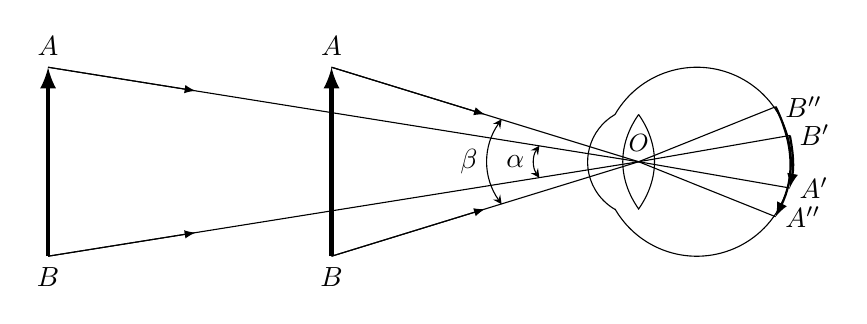
\begin{tikzpicture}[>=latex, scale=1.2]
    % eye begin
    \draw (0,.5) arc (150:-150:1);
    \draw (0,.5) arc (120:240:.58);
    \draw (0.25,.5)to [bend left=35] (.25,-.5)to [bend left=35](0.25,.5) ;
    % eye end

\draw[->, ultra thick] (-6,-1)node[below]{$B$}--(-6,1)node[above]{$A$};
\draw[->, ultra thick] (-3,-1)node[below]{$B$}--(-3,1)node[above]{$A$};

\draw (-3,-1)--(0.25,0)--(1.7, .582)node[right]{$B''$};
\draw (-3, 1)--(0.25,0)--(1.7, -.582)node[right]{$A''$};
\draw (-6,-1)--(0.25,0)--(1.85, .278)node[right]{$B'$};
\draw (-6,1)--(0.25,0)--(1.85, -.278)node[right]{$A'$};

\draw [->, thick](1.7, .582)to [bend right=-26] (1.7, -.582);
\draw [->,  thick](1.85, .278)to [bend right=-11] (1.85, -.278);

\node at (0.25,0)[above]{\small $O$};

\draw[->] (-3,-1)--(-2.75/2,-.5);
\draw[->] (-3, 1)--(-2.75/2,.5);
\draw[->] (-6,-1)--(-4.4375,-.75);
\draw[->] (-6,1)--(-4.4375,.75);

\draw [<->, >=stealth](-1.2, .45)to [bend left=-35]node[left]{$\beta$} (-1.2, -.45);
\draw [<->, >=stealth](-.8, .17)to [bend left=-35]node[left]{$\alpha$} (-.8, -.17);


\end{tikzpicture}
    \caption{物体离眼睛近时视角大}
    \end{figure}

如果物体在视网膜上的像小到只落在一个感光细胞上,
那么眼睛看到的就只是一个点。要使眼睛把物体上的两个点
区分开,必须使这两个点在视网膜上的像落在不同的感光细
胞上。这样,这两个点的视角就必须大于某一数值才行。根
据实验知道,正常眼的这一数值约等于1分($1'$),大小为0.1
毫米的物体,在离眼睛25厘米的明视距离处,所成的视角大
约就是$1'$。

把物体移得离眼睛近些可以增大视角,使眼睛看清物体,
但是这种方法是有一定限度的,物体移到近点以后就不能再
移近了。有些物体(例如天体)无法移近眼睛,不能用这种办
法来增大视角。在这些情况下,为了看清物体,就需要借助于
显微镜、望远镜等光学仪器。

\section{显微镜和望远镜}
\subsection{显微镜}

观察细菌、动植物的组织、金属的结构等细微物
体,要用显微镜。显微镜能把物体放大很多倍,下面我们来说
明它的原理。

显微镜的主要部分是装在
镜筒两端的两组透镜,每组透
镜都相当于一个凸透镜。靠近
被观察物体的一组透镜叫做\textbf{物
镜},靠近眼睛的一组透镜叫做
\textbf{目镜}。物镜的焦距很短,目镜的
焦距较长。

物镜的作用是得到被观察
物体的放大的实像,目镜的作
用是把物镜所成的实像作为物
体,一步把它放大为虚像。

\begin{figure}[htp]\centering
    \includegraphics[scale=.6]{fig/5-53.png}
    \caption{显微镜的成像光路图}
    \end{figure}

图5.53是显微镜的成像光路图.物镜$L_1$到被观察物$AB$
的距离稍大于物镜的焦距$f_1$,通过物镜得到放大的实像$A'B'$。
$A'B'$对目镜$L_2$来说是物体,使$A'B'$位于目镜的焦点$F_2$以内,
这样通过目镜就得到$A'B'$的放大的虚像$A''B''$。从图上可以
看出,$A''B''$的视角比眼睛直接看$AB$时的视角大得多。所以
用显微镜可以看清非常微小的物体。

人眼只能看清大小为0.1毫米左右的细节,光学显微镜
的放大率为1000—1500倍左右,可使我们看清物体万分之一
毫米左右的细微结构,大大提高了我们的观察能力,但是要
观察物质更细微的构造,例如晶体的结构、分子、原子等,光学
显微镜就无能为力了,必须用放大率更高的电子显微镜。

\subsection{望远镜}

观察远处的物体或天体要用望远镜。望远镜的
构造有不同的型式,下面我们介绍开普勒望远镜和反射式望
远镜。

开普勒望远镜是德国天文学家开普勒在1611年发明的,
主要用来观察天体,所以叫做天文望远镜,它由两组透镜组
成,每组透镜都相当于一个凸透镜,其中对着远处物体的一组
叫做物镜,对着眼睛的一组叫做目镜。但是跟显微镜相反,望
远镜的物镜焦距较长,目镜焦距较短。
\begin{figure}[htp]\centering
    \includegraphics[scale=.6]{fig/5-54.png}
    \caption{开普勒望远镜原理图}
    \end{figure}

开普勒望远镜的原理如图5.54所示。从天体射来的平
行光线,经过物镜$L_1$后,在焦点以外距焦点很近的地方成一
倒立缩小的实像$A'B'$。目镜$L_2$的前焦点和物镜的焦点是重
合的,所以实像$A'B'$位于$L_2$和它的焦点之间距焦点很近的
地方,$L_2$以$A'B'$为物体,形成放大的虚像$A''B''$.这样,当
我们对着目镜观察的时候,进入眼睛的光线就好象是从$A''B''$
射来的。$A''B''$的视角大于直接用眼睛观察天体时的视角,因
此从望远镜中看到的物体使人觉得离自己近了,看得清楚了。

望远镜的物镜越大,进入镜中的光就越多,所成的像就越
明亮清晰,这对于观察传来的光很弱的遥远星体是很重要的。
但是由于制造和安装上的困难,透镜的直径很难大于1米,所
以天文台用的大型望远镜多为反射式的。这种望远镜是牛顿
在1668年发明的。反射式望远镜的原理如图5.55所示。它
用一个很大的凹镜代替物镜,从遥远天体射来的平行光线,经
凹镜$C$反射后,向焦点会聚,但是在光线还没有会聚到焦点以
前,就被平面镜$M$反射到目镜$O$中,形成实像。反射式望远镜
的凹镜可以做得很大,能够集中较多的光,使成像明亮清晰。
凹镜的口径越大,能够看到的宇宙范围也就越大,现在世界
上已有口径为5米的反射式望远镜。
\begin{figure}[htp]\centering
    \includegraphics[scale=.6]{fig/5-55.png}
    \caption{反射式望远镜原理图}
    \end{figure}

\section*{阅读材料:电子显微镜和射电望远镜}
\subsection*{电子显微镜}

    \begin{figure}[htp]
        \centering
        \begin{minipage}[t]{0.48\textwidth}
        \centering
        \includegraphics[scale=.6]{fig/5-56.png}
        \end{minipage}
        \begin{minipage}[t]{0.48\textwidth}
        \centering
        \includegraphics{fig/5-56.pdf}
        \end{minipage}
        \caption{用磁场聚焦的电子显微镜的示意图(右图)}
        \end{figure}

电子显微镜是在本世纪三十年代出现的。
它是类比于光学显微镜发展起来的,光学显徽镜是用可见光照射被研究的物体,利用光学透镜使光线偏折而成像的;电子
显微镜则是让电子束穿过被研究的物体,利用电磁透镜(实际
上就是按一定要求分布的空间电场和磁场)使电子束偏转而
成像的,图5.56是用磁场聚焦的电子显微镜的示意图,
为了便于类比,左边画出了光学显微镜的示意图。发射电子
的阴极$K$相当于光学显微镜的光源,从阴极发射出来的电子,
经过磁透镜$L_1$后变为平行的电子束,$L_1$起聚光镜的作用,电
子束穿过被研究的物体$O$,产生被研究物体的透射像。磁透镜$L_2$起物镜的作用,电子束通过它,放大成像$I_1$,$I_1$再经磁透镜$L_3$放大,第二次成像$I_2$。$I_2$被投射在荧光屏$S$上,可以用
照相方法记录下来。


电子显微镜的放大率比光学显微镜的放大率高一千倍左
右,电子显微镜能观察物质的精细结构,可以拍摄出物质的
原子结构图,在现代科学技术中有重要的应用。

\subsection*{射电望远镜}
太阳、恒星和宇宙空间的物质能发出无线
电波,这种无线电波叫做射电辐射,观测射电辐射的强度,是
天文学中研究天体和宇宙的一种重要方法。射电望远镜就是
用来观测宇宙中射电辐射的仪器。
\begin{figure}[htp]\centering
    \includegraphics[scale=1]{fig/5-57.pdf}
    \caption{射电望远镜}
    \end{figure}

射电望远镜有各式各样的结构,图5.57所示的是常见的
抛物面天线射电望远镜,它有一个很大的金属抛物面状天线,
从宇宙空间射来的平行于抛物面轴的无线电波,被反射后集
中到位于抛物面焦点处的小天线上,小天线接收到的无线电
波能量通过传输线输送给接收机,接收机对电波能量进行测
量,确定射电波的强度。

利用射电望远镜进行观测有许多优点。无线电波能穿过
云雾和尘埃,因此用射电望远镜能不分晴雨昼夜连续进行观
测;对于那些难以用光学望远镜观测的天体和字宙空间,利用
射电望远镜也可以进行研究。

\section*{复习题}
\begin{enumerate}
\item 什么叫做光线?举例说明哪些现象是光沿直线传播
而产生的?
\item 什么叫光的反射?光的反射定律的内容是什么?
\item 平面镜、凹镜、凸镜各对光线起什么作用?它们的成
像情况有什么不同?
\item 什么叫光的折射?光的折射定律的内容是什么?什么
叫媒质的绝对折射率?什么叫一种媒质对另一种媒质的相对
折射率?它们跟光速的关系是怎样的?
\item 什么叫全反射现象?付么叫临界角?举两个全反射现
象的例子。
\item 射向玻璃棱镜侧面的光线,通过棱镜后,为什么向底
面偏折?什么现象表明在同种媒质中各种色光的折射率不
同?紫光的折射率大,还是红光的折射率大?
\item 凸透镜为什么能使光线会聚?凹透镜为什么能使光
线发散?为什么说凸透镜的焦点是实焦点,而凹透镜的是虚焦
点?
\item 说明凸透镜和凹透镜的成像规律。用作图法求像时
为什么要利用三条特殊光线?像是不是仅由这三条特殊光线
形成的?

写出透镜成像的公式。在应用这个公式时应注意什么?
怎样计算像的放大率?
\item 眼睛为什么能使远处的物体和近处的物体都成像在
视网膜上?近视眼和远视眼跟正常眼的差别各是什么?它们各
应戴什么眼镜?
\item 什么叫视角?为什么观察物体时视角越大看得越清
楚?
\item 说明显微镜的构造和作用,画出它的成像光路图。
\item 说明开普勒望远镜和反射式望远镜的构造和原理。

\end{enumerate}

\section*{习题}
\begin{enumerate}
    \item 为了使身高1.8米的人能从平面镜中看到自己的全
身像,如果镜和人都是直立的,平面镜的长度至少应为多长?
画图加以说明。
\item 光可以从弯曲玻璃棒的一端传到另一端,这是否跟
光在同一种媒质中沿直线传播相矛盾?
\item 在水面下1.0米处有一个点光源,从水面上看,这个
点光源能照亮水面多大的面积?
\item 用下面的方法可以测量液体的折射率:取一个半径
为$r$的软木塞,在它的圆心处插上一枚大头针,让软木塞浮在
液面上(图5.58)。调整大头针插进软木塞的深度,使它露在
外面的长度为$h$。这时从软木塞周围各个方向向液体中看,恰
好看不到大头针。利用测得的数据$r$和$h$即可以求出液体的
折射率。
\begin{enumerate}
    \item 写出用$r$和$h$求折射率的计算式;
    \item 用这种方法实际做一下,求出水的折射率。
\end{enumerate}
\begin{figure}[htp]\centering
    \includegraphics[scale=1]{fig/5-58.pdf}
    \caption{}
    \end{figure}
\item 为了从坦克内部观察外界目标,在坦克壁上开有一
个长方形孔。假定坦克的壁厚为20厘米,孔的宽度为12厘
米,孔内安装一块折射率$n=1.52$的玻璃,厚度跟坦克的壁厚
相同,车内人员通过这块玻璃能看到的外界范围为多大角度?
\item 图5.59中给出了光线在光学器件上射入和射出的
方向,试在方框内画出可用的光学器件及光路图。
\begin{figure}[htp]
	\centering
\begin{tikzpicture}[>=latex]
  
\draw (0,0) rectangle (1.5,1.5);
\draw (0,2.5) rectangle (0+1.5,2.5+1.5);
\draw (4,0) rectangle (4+1.5,1.5);
 \draw (4,2.5) rectangle (4+1.5,2.5+1.5);
\draw [->] (5.5, 1.3)--(6.5,1.3);
\draw [->] (5.5, .2)--(6.5,.2);
\draw [->] (3, 1)--(4,1);
\draw [->] (3, .5)--(4,.5);


\draw [->] (5.5, 3.8)--(6.5,3.8);
\draw [->] (5.5, 2.7)--(6.5,2.7);
\draw [->] (3, 3.5)--(4,3);
\draw [->] (3, 3)--(4,3.5);

\draw [->] (-1, 3.5)--(0,3.5);
\draw [->] (-1, 3)--(0,3);
\draw [->] (.5, 4)--(.5,5);
\draw [->] (1, 4)--(1,5);

\draw [->] (-1, 1.3)--(0,1.3);
\draw [<-] (-1, .2)--(0,.2);
\draw [->] (-1, 1.1)--(0,1.1);
\draw [<-] (-1, .4)--(0,.4);

\end{tikzpicture}
	\caption{}
\end{figure}
\item 如果把凸透镜的中部用一块黑纸遮住,用它还能得
到物体的像吗?为什么?
\item 蜡烛到凸透镜的距离为20厘米,到光屏的距离为40
厘米,这时在光屏上得到清晰的烛像,如果把凸透镜向光屏
移动5厘米,光屏应向后移动多远才能再得到清晰的烛像?这
时像的放大率是增大了,还是减小了?
\item 当物体到凸透镜的距离为36厘米时,光屏上所成的
像的高度为10厘米;当物体到凸透镜的距离变为24厘米时,
光屏上像的高度变为20厘米,这个凸透镜的焦距是多大?
\item 透镜焦距的倒数$1/f$
叫做透镜的焦度,焦度的单位叫
做屈光度,透镜的焦距为1米时,焦度为1屈光度。屈光度
乘以100,就是通常所说的眼镜的度数,某同学眼镜的近视度
数是250度,他的眼镜是什么透镜?焦距是多大?
\item 如图5.60所示,如果以凸透镜的两个焦点$F_1$、$F_2$
分别作为计算物距和像距的起点,并且用x表示物体AB到
第一焦点$F_1$的距离,以$x'$表示像$A'B'$到第二焦点$F_2$的距
离。试证明;凸透镜成像的公式
\[\frac{1}{u}+\frac{1}{v}=\frac{1}{f} \]
将变为$xx'=f^2$。此式称为牛顿薄透镜公式,在光学书中经常遇到。
\begin{figure}[htp]
	\centering
\begin{tikzpicture}
  \draw [dash dot](-4,0)--(5,0);
\fill (-2,0) circle (1.5pt) node[below]{$F_1$};
\fill (2.5,0) circle (1.5pt)node[above]{$F_2$};
\draw[->, very thick, -latex](-3.5,0)node[below]{$B$}--(-3.5,.8)node[above]{$A$};
\draw[->, very thick, -latex](4.5,0)node[above]{$B'$}--(4.5,-1.5)node[below]{$A'$};
\draw[<->, ultra thick ](0,2)--(0,-2);
\node at (.25,.25){$O$};
\draw[ stealth-stealth](-3.5,.4)--node [fill=white]{$x$}(-2,.4);
\draw[ stealth-stealth](4.5,-.4)--node [fill=white]{$x'$}(2.5,-.4);
\draw (-2,0)--(-2,.5); \draw (2.5,0)--(2.5,-.6); 
\end{tikzpicture}
	\caption{}
\end{figure}
(提示:$u=x+f$,$v=x'+f$)
\item 某人用焦距为2厘米和8厘米的两个凸透镜分别
作物镜和目镜,制成一架简易显微镜。如果物镜到被观察物
体的距离为2.2厘米,要想使目镜最后所成的虚像距目镜25
厘米,目镜和物镜间的距离应为多大?这架显微镜的放大率是
多大?
\end{enumerate}





























































